\documentclass[aspectratio=169,10pt]{beamer}
\usepackage[utf8]{inputenc}
\usepackage[T5]{fontenc}
\usepackage[vietnamese]{babel}
\usepackage{graphicx}
\usepackage{hyperref}
\usepackage{lmodern}
\usepackage{booktabs}
\usepackage{amsmath,amssymb}
\usepackage{colortbl}

% Color Theme - Nông nghiệp Công nghệ cao (Forest Green & Deep Emerald)
\definecolor{AgriPrimary}{RGB}{20, 83, 45}     % #14532d
\definecolor{AgriSecondary}{RGB}{22, 101, 52}  % #166534
\definecolor{AgriAccent}{RGB}{34, 197, 94}     % #22c55e
\definecolor{AgriDark}{RGB}{15, 23, 42}        % #0f172a
\definecolor{AgriBg}{RGB}{248, 250, 252}       % #f8fafc

\usetheme{Madrid}
\usecolortheme{whale}

\setbeamercolor{palette primary}{bg=AgriPrimary,fg=white}
\setbeamercolor{palette secondary}{bg=AgriSecondary,fg=white}
\setbeamercolor{palette tertiary}{bg=AgriPrimary!80!black,fg=white}
\setbeamercolor{titlelike}{bg=AgriPrimary,fg=white}
\setbeamercolor{block title}{bg=AgriSecondary,fg=white}
\setbeamercolor{block body}{bg=AgriPrimary!5,fg=AgriDark}
\setbeamercolor{block title example}{bg=AgriAccent!80!black,fg=white}
\setbeamercolor{block body example}{bg=AgriAccent!10,fg=AgriDark}
\setbeamercolor{block title alerted}{bg=red!75!black,fg=white}
\setbeamercolor{block body alerted}{bg=red!5,fg=AgriDark}

\title[Ôn tập AI trong Nông nghiệp]{ỨNG DỤNG AI TRONG NÔNG NGHIỆP}
\subtitle{BÁO CÁO TỔNG KẾT \& TÓM TẮT NỘI DUNG 10 BUỔI HỌC}
\author[Khoa CNTT - ĐH Đông Á]{Bộ môn Trí tuệ Nhân tạo \& Nông nghiệp Số}
\institute[UDA]{Trường Đại học Đông Á (UDA)}
\date{\today}

\begin{document}

% ==========================================
% SLIDE 1: TRANG TIÊU ĐỀ
% ==========================================
\begin{frame}
    \titlepage
\end{frame}

% ==========================================
% SLIDE 2: LỘ TRÌNH 10 BUỔI HỌC
% ==========================================
\begin{frame}{Lộ trình môn học: 10 Buổi kiến tạo Nông nghiệp 4.0}
    \begin{columns}[c]
        \begin{column}{0.55\textwidth}
            \textbf{4 Trụ cột chuyên môn cốt lõi:}
            \begin{enumerate}
                \item \textbf{Nền tảng \& Thuật toán}: AI tổng quan, Machine Learning, Deep Learning (Buổi 1--3).
                \item \textbf{Thị giác \& Hệ chuyên gia}: Computer Vision, Cây quyết định DSS nông hộ (Buổi 4--5).
                \item \textbf{Tài nguyên \& Hoạch định}: Quản lý tưới tiêu, IoT, Dự báo năng suất cây trồng (Buổi 6--7).
                \item \textbf{Dự án \& Triển khai thực tế}: Quản lý dự án ML, Edge AI, Drone, Thực hành trang trại (Buổi 8--10).
            \end{enumerate}
        \end{column}
        \begin{column}{0.42\textwidth}
            \centering
            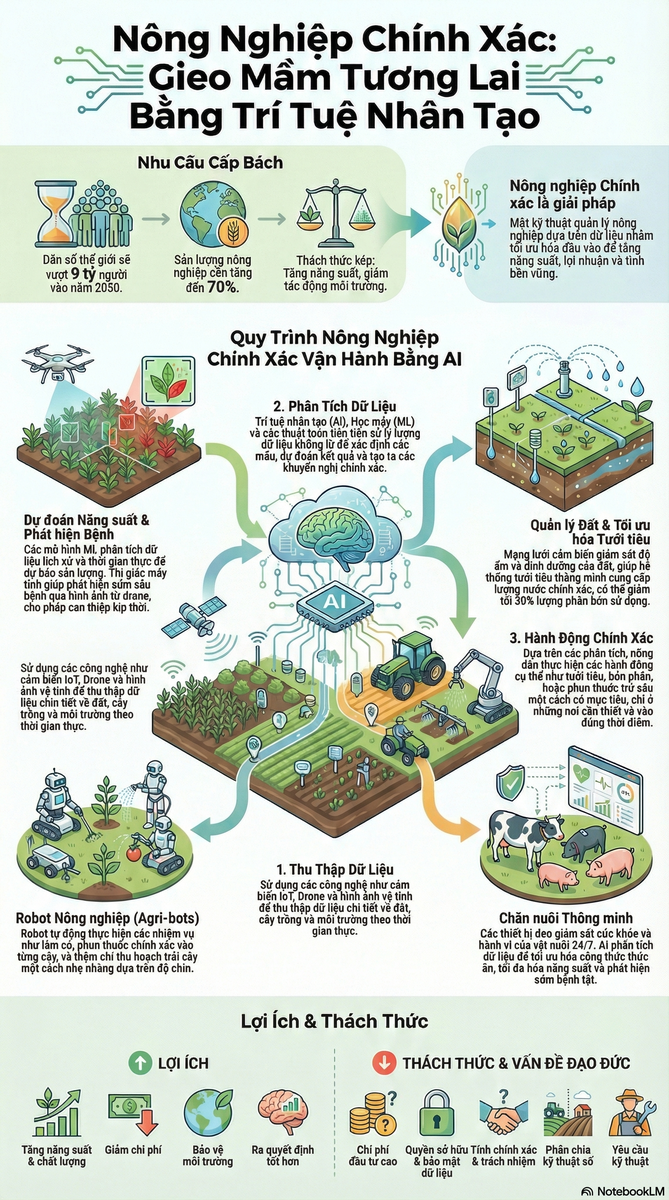
\includegraphics[width=\linewidth,height=0.72\textheight,keepaspectratio]{images_ontap/b1_infographic.png}
        \end{column}
    \end{columns}
\end{frame}

% ==========================================
% SLIDE 3: MỤC LỤC CHI TIẾT
% ==========================================
\begin{frame}{Nội dung ôn tập trọng tâm}
    \begin{columns}[t]
        \begin{column}{0.48\textwidth}
            \begin{block}{Phần I: Nền tảng \& Thuật toán (B1--B4)}
                \begin{itemize}
                    \item \textbf{Buổi 1}: Tổng quan AI, Nông nghiệp chính xác.
                    \item \textbf{Buổi 2}: Học máy (ML), phân loại đất, khuyến nghị.
                    \item \textbf{Buổi 3}: Học sâu (DL), CNN chẩn đoán bệnh lá.
                    \item \textbf{Buổi 4}: Thị giác máy tính, phát hiện sâu bệnh.
                \end{itemize}
            \end{block}
            \begin{block}{Phần II: Hệ chuyên gia \& Giữa kỳ (B5)}
                \begin{itemize}
                    \item \textbf{Buổi 5}: Hệ DSS cà phê, hồ tiêu, sầu riêng, đất.
                \end{itemize}
            \end{block}
        \end{column}
        \begin{column}{0.48\textwidth}
            \begin{block}{Phần III: Quản lý \& Hoạch định (B6--B7)}
                \begin{itemize}
                    \item \textbf{Buổi 6}: IoT, Tưới tiêu DRL, cân bằng NPK.
                    \item \textbf{Buổi 7}: Dữ liệu lớn, Viễn thám NDVI, Dự báo.
                \end{itemize}
            \end{block}
            \begin{block}{Phần IV: Dự án \& Thực chiến (B8--B10)}
                \begin{itemize}
                    \item \textbf{Buổi 8}: Báo cáo dự án, Đạo đức, Checklist.
                    \item \textbf{Buổi 9}: Công cụ lập trình (Python, TF, OpenCV).
                    \item \textbf{Buổi 10}: Huấn luyện mô hình, Edge AI.
                \end{itemize}
            \end{block}
        \end{column}
    \end{columns}
\end{frame}

% ==========================================
% SLIDE 4: BUỔI 1 - TỔNG QUAN AI
% ==========================================
\begin{frame}{Buổi 1: Tổng quan AI \& Cuộc cách mạng Nông nghiệp 4.0}
    \begin{columns}[c]
        \begin{column}{0.55\textwidth}
            \begin{block}{Bối cảnh và Động lực}
                \begin{itemize}
                    \item Dân số thế giới dự báo đạt 9.7 tỷ người vào 2050 $\rightarrow$ nhu cầu lương thực tăng 60--70\%.
                    \item Biến đổi khí hậu, cạn kiệt tài nguyên nước, suy thoái đất.
                \end{itemize}
            \end{block}
            \begin{block}{Vai trò của Trí tuệ Nhân tạo (AI)}
                \begin{itemize}
                    \item Chuyển đổi từ \textit{"kinh nghiệm cảm tính"} sang \textit{"canh tác dựa trên dữ liệu"}.
                    \item Tự động hóa quy trình: tưới tiêu, bón phân, phun thuốc.
                    \item Nâng cao năng suất cây trồng và tối ưu chi phí đầu vào.
                \end{itemize}
            \end{block}
        \end{column}
        \begin{column}{0.42\textwidth}
            \centering
            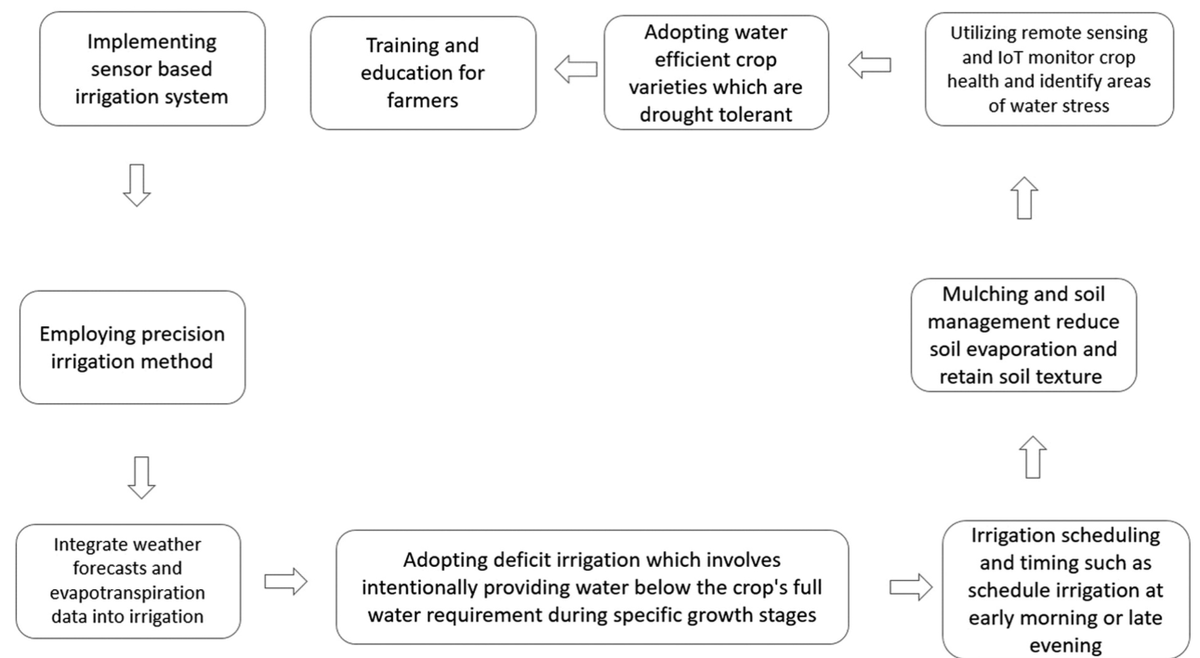
\includegraphics[width=\linewidth,height=0.72\textheight,keepaspectratio]{images_ontap/b1_precision.png}
            \vspace{0.2cm}
            \footnotesize{\textit{Hệ sinh thái Nông nghiệp Thông minh}}
        \end{column}
    \end{columns}
\end{frame}

% ==========================================
% SLIDE 5: BUỔI 1 - NÔNG NGHIỆP CHÍNH XÁC
% ==========================================
\begin{frame}{Buổi 1: Nông nghiệp Chính xác (Precision Agriculture)}
    \begin{columns}[c]
        \begin{column}{0.55\textwidth}
            \textbf{Nguyên tắc 4 Đúng (4R of Nutrient Management):}
            \begin{itemize}
                \item \textbf{Đúng vị trí} (Right Place): Canh tác theo biến thiên thổ nhưỡng.
                \item \textbf{Đúng liều lượng} (Right Rate): Cấp đủ lượng cây cần, không dư thừa.
                \item \textbf{Đúng thời điểm} (Right Time): Cấp theo giai đoạn sinh trưởng.
                \item \textbf{Đúng chủng loại} (Right Source): Dạng phân bón/nước tối ưu.
            \end{itemize}
            \vspace{0.2cm}
            \begin{alertblock}{Mắt xích công nghệ}
                IoT Sensors + Drone/UAV + AI Analytics $\rightarrow$ VRA (Variable Rate Application).
            \end{alertblock}
        \end{column}
        \begin{column}{0.42\textwidth}
            \centering
            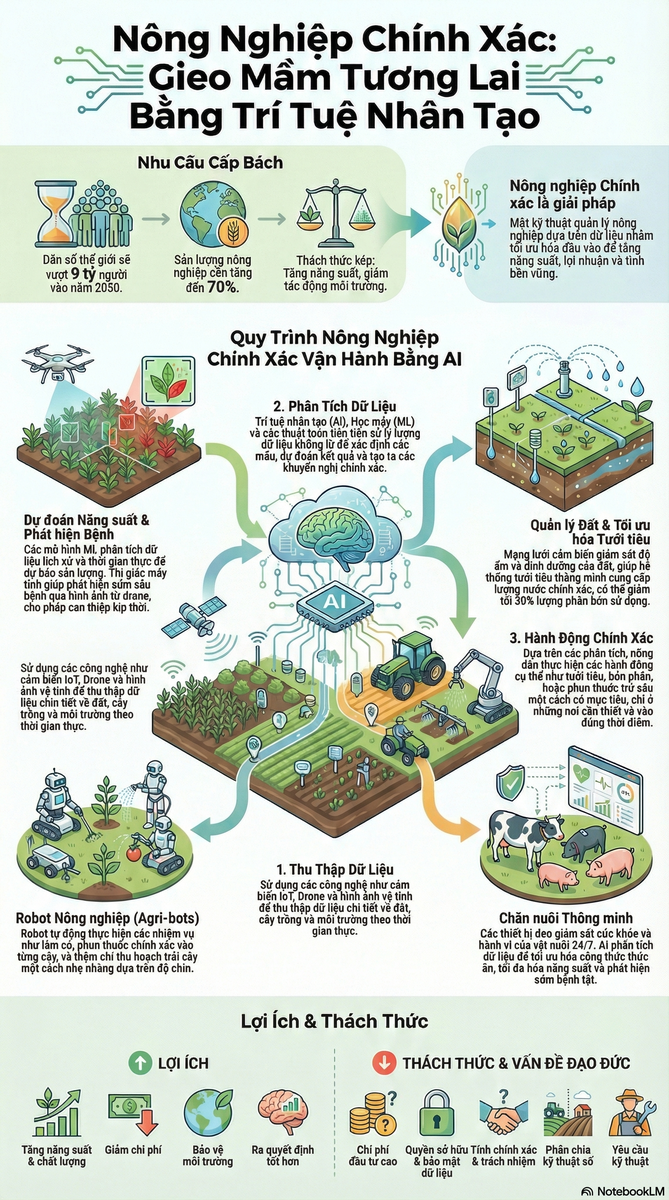
\includegraphics[width=\linewidth,height=0.72\textheight,keepaspectratio]{images_ontap/b1_infographic.png}
        \end{column}
    \end{columns}
\end{frame}

% ==========================================
% SLIDE 6: BUỔI 1 - ĐẠO ĐỨC & TRÁCH NHIỆM AI
% ==========================================
\begin{frame}{Buổi 1: Đạo đức, Thách thức \& Responsible AI}
    \begin{columns}[c]
        \begin{column}{0.55\textwidth}
            \begin{block}{Các thách thức cốt lõi}
                \begin{itemize}
                    \item \textbf{Quyền sở hữu dữ liệu}: Dữ liệu đồng ruộng thuộc về nông dân hay nhà cung cấp giải pháp AI?
                    \item \textbf{Thiên lệch dữ liệu (Data Bias)}: Mô hình huấn luyện ở ôn đới khó áp dụng chuẩn xác cho nhiệt đới.
                    \item \textbf{Chi phí \& Rào cản số}: Đảm bảo nông hộ nhỏ lẻ có thể tiếp cận công nghệ giá rẻ.
                \end{itemize}
            \end{block}
            \begin{exampleblock}{Nguyên tắc Responsible AI}
                Minh bạch (Transparency), Công bằng (Fairness), Bảo mật (Privacy) và Bền vững (Sustainability).
            \end{exampleblock}
        \end{column}
        \begin{column}{0.42\textwidth}
            \centering
            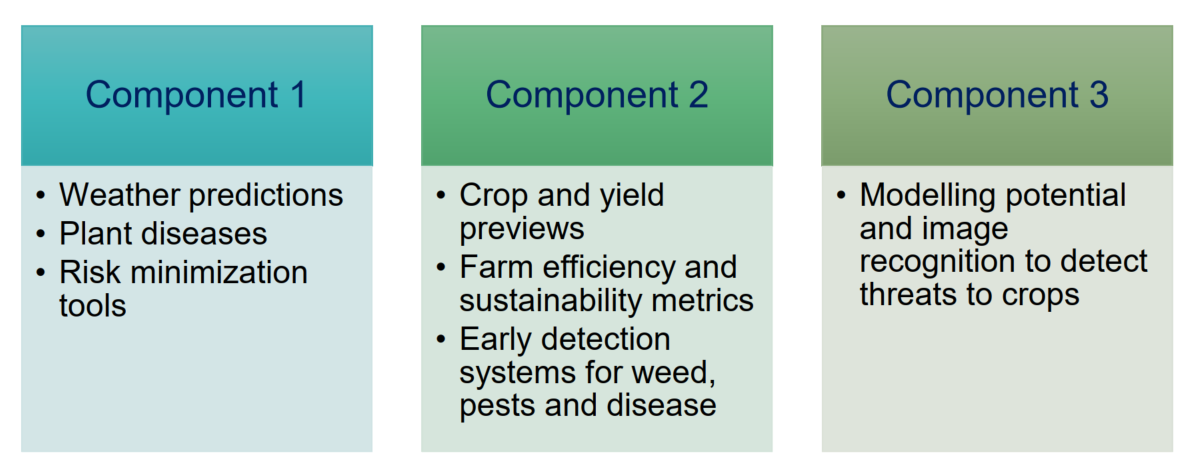
\includegraphics[width=\linewidth,height=0.72\textheight,keepaspectratio]{images_ontap/b1_ethics.png}
            \vspace{0.2cm}
            \footnotesize{\textit{Khung đạo đức AI trong nông nghiệp}}
        \end{column}
    \end{columns}
\end{frame}

% ==========================================
% SLIDE 7: BUỔI 2 - HỌC MÁY TRONG NÔNG NGHIỆP
% ==========================================
\begin{frame}{Buổi 2: Học máy (Machine Learning) - 3 Phân nhánh chính}
    \begin{columns}[c]
        \begin{column}{0.55\textwidth}
            \textbf{Phân loại các phương pháp Học máy:}
            \begin{itemize}
                \item \textbf{Học có giám sát (Supervised Learning)}:
                \begin{itemize}
                    \item Dữ liệu có nhãn $(X, y)$.
                    \item \textit{Phân loại}: Bệnh lá, loại đất, phát hiện sâu.
                    \item \textit{Hồi quy}: Dự báo năng suất vụ mùa, nhiệt độ.
                \end{itemize}
                \item \textbf{Học không giám sát (Unsupervised Learning)}:
                \begin{itemize}
                    \item Dữ liệu không nhãn. Phân cụm (Clustering K-Means) vùng đất đồng nhất, phân khúc nông sản.
                \end{itemize}
                \item \textbf{Học tăng cường (Reinforcement Learning)}:
                \begin{itemize}
                    \item Tác tử học qua thưởng/phạt: Tưới tiêu tự động, robot gieo hạt.
                \end{itemize}
            \end{itemize}
        \end{column}
        \begin{column}{0.42\textwidth}
            \centering
            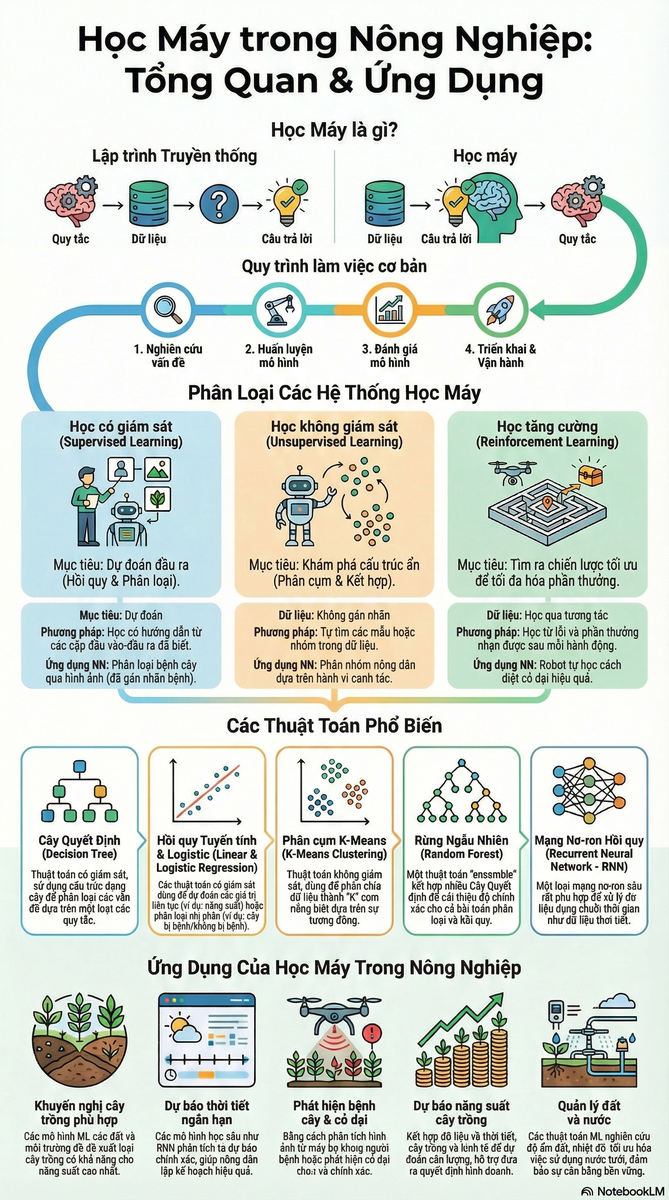
\includegraphics[width=\linewidth,height=0.72\textheight,keepaspectratio]{images_ontap/b2_infographic.png}
        \end{column}
    \end{columns}
\end{frame}

% ==========================================
% SLIDE 8: BUỔI 2 - THUẬT TOÁN KINH ĐIỂN
% ==========================================
\begin{frame}{Buổi 2: Thuật toán ML kinh điển \& Khuyến nghị Cây trồng}
    \begin{columns}[c]
        \begin{column}{0.55\textwidth}
            \begin{block}{Các thuật toán thường dùng}
                \begin{itemize}
                    \item \textbf{Decision Tree \& Random Forest}: Dễ giải thích, xử lý tốt dữ liệu phi tuyến (độ ẩm, pH, NPK).
                    \item \textbf{SVM (Support Vector Machine)}: Hiệu quả cao khi số chiều lớn, dữ liệu mẫu nhỏ.
                    \item \textbf{KNN (K-Nearest Neighbors)}: Phân loại thổ nhưỡng cục bộ.
                \end{itemize}
            \end{block}
            \begin{exampleblock}{Bài toán Crop Recommender}
                Đầu vào: $[N, P, K, \text{pH}, \text{Nhiệt độ}, \text{Độ ẩm}, \text{Lượng mưa}] \rightarrow$ Đầu ra: Cây trồng thích hợp nhất (Lúa, Cà phê, Ngô, Đậu).
            \end{exampleblock}
        \end{column}
        \begin{column}{0.42\textwidth}
            \centering
            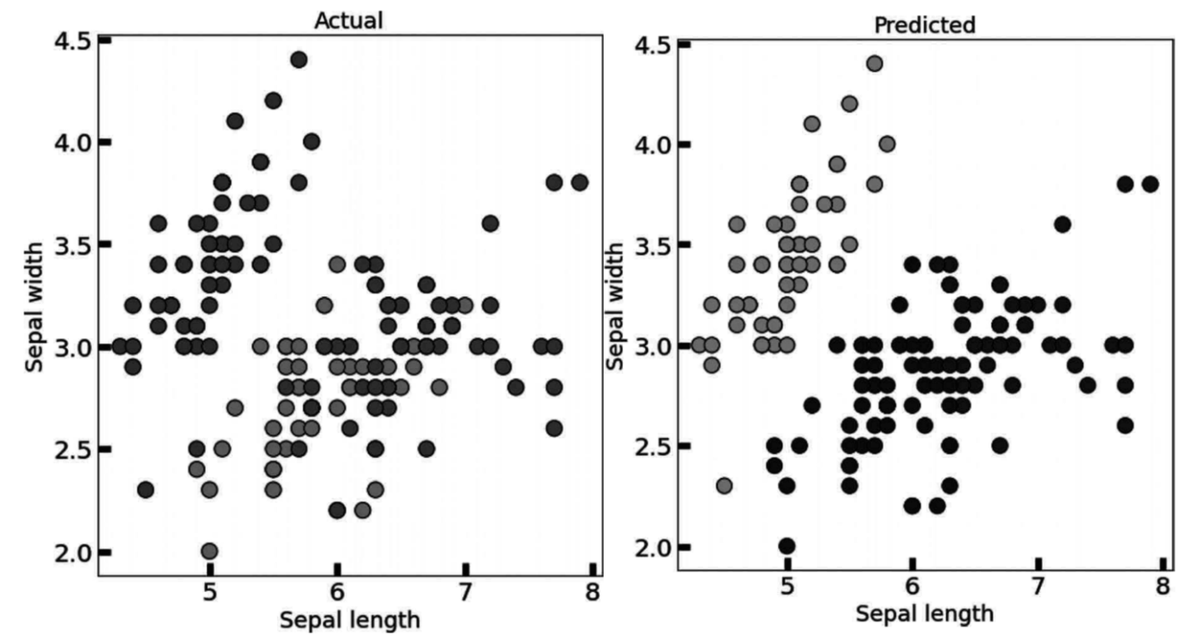
\includegraphics[width=\linewidth,height=0.72\textheight,keepaspectratio]{images_ontap/b2_crop_recom.png}
            \vspace{0.2cm}
            \footnotesize{\textit{Cây quyết định trong khuyến nghị nông nghiệp}}
        \end{column}
    \end{columns}
\end{frame}

% ==========================================
% SLIDE 9: BUỔI 2 - QUY TRÌNH HUẤN LUYỆN ML
% ==========================================
\begin{frame}{Buổi 2: Pipeline chuẩn phát triển mô hình ML Nông nghiệp}
    \begin{columns}[c]
        \begin{column}{0.55\textwidth}
            \textbf{6 Bước thực thi chuẩn hóa:}
            \begin{enumerate}
                \item \textbf{Thu thập dữ liệu}: Cảm biến IoT, số liệu khí tượng, nhật ký canh tác.
                \item \textbf{Làm sạch \& Tiền xử lý}: Xử lý missing data, khử nhiễu cảm biến, chuẩn hóa thang đo (MinMax, StandardScaler).
                \item \textbf{Kỹ thuật đặc trưng (Feature Engineering)}: Trích xuất chỉ số tương quan, độ ẩm tích lũy.
                \item \textbf{Huấn luyện mô hình}: Chia tập Train/Val/Test (70/15/15), K-fold Cross Validation.
                \item \textbf{Đánh giá}: $R^2$, RMSE, MAE (Hồi quy); Precision, Recall, F1-Score (Phân loại).
                \item \textbf{Triển khai}: Đóng gói API, Dashboard theo dõi.
            \end{enumerate}
        \end{column}
        \begin{column}{0.42\textwidth}
            \centering
            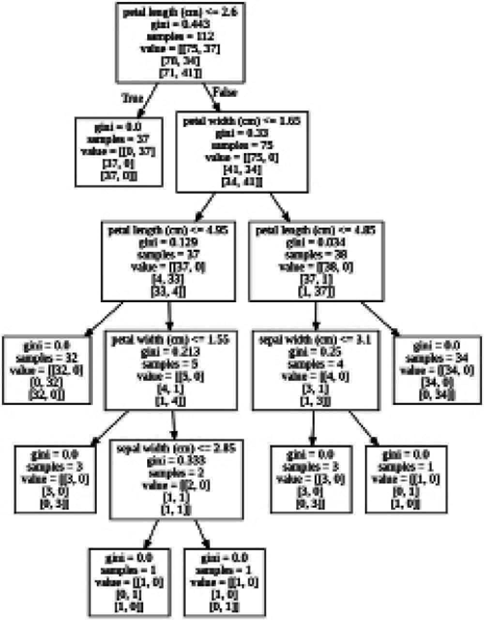
\includegraphics[width=\linewidth,height=0.72\textheight,keepaspectratio]{images_ontap/b2_algorithms.png}
            \vspace{0.2cm}
            \footnotesize{\textit{Ma trận phân cụm và tương quan đặc trưng}}
        \end{column}
    \end{columns}
\end{frame}

% ==========================================
% SLIDE 10: BUỔI 3 - HỌC SÂU & MẠNG NƠ-RON
% ==========================================
\begin{frame}{Buổi 3: Học sâu (Deep Learning) \& Mạng Nơ-ron nhân tạo}
    \begin{columns}[c]
        \begin{column}{0.55\textwidth}
            \begin{block}{Tại sao cần Deep Learning trong Nông nghiệp?}
                \begin{itemize}
                    \item ML truyền thống gặp giới hạn khi xử lý dữ liệu phi cấu trúc lớn (Ảnh lá cây, Video camera, Ảnh vệ tinh).
                    \item DL tự động học các biểu diễn phân cấp (Representation Learning) mà không cần Feature Engineering thủ công.
                \end{itemize}
            \end{block}
            \begin{block}{Kiến trúc Mạng nơ-ron cơ bản}
                \begin{itemize}
                    \item \textbf{Perceptron \& MLP (Multilayer Perceptron)}: Tầng vào $\rightarrow$ Các tầng ẩn (Hidden Layers) $\rightarrow$ Tầng ra.
                    \item Hàm kích hoạt phi tuyến: ReLU, Sigmoid, Softmax.
                \end{itemize}
            \end{block}
        \end{column}
        \begin{column}{0.42\textwidth}
            \centering
            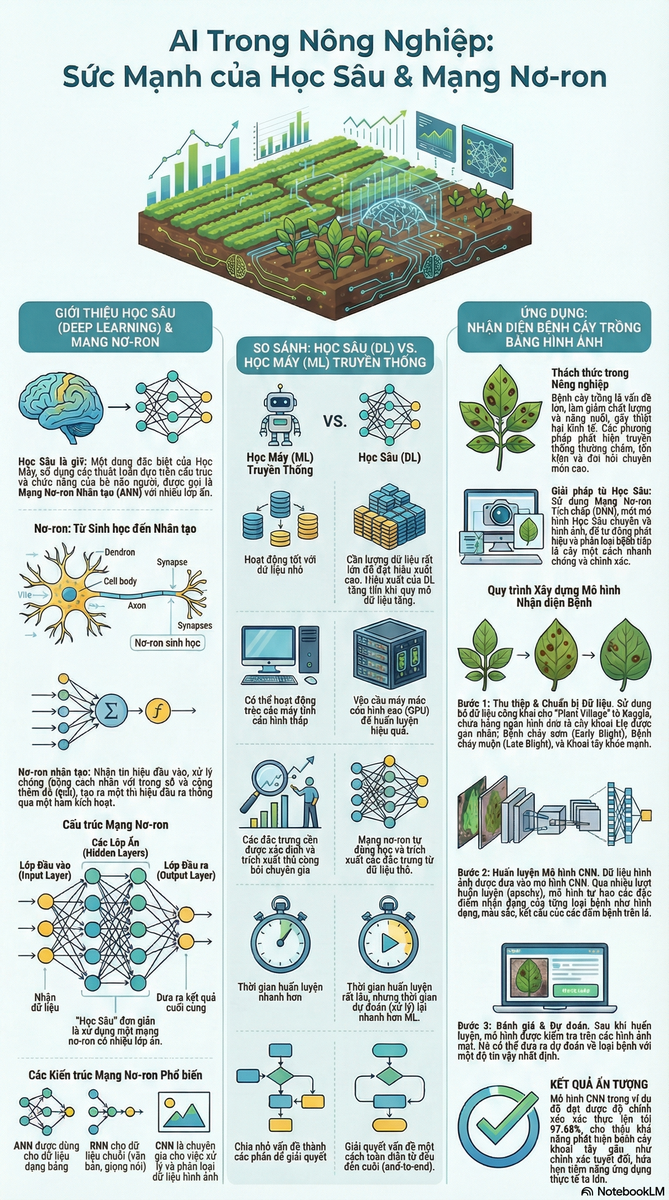
\includegraphics[width=\linewidth,height=0.72\textheight,keepaspectratio]{images_ontap/b3_infographic.png}
        \end{column}
    \end{columns}
\end{frame}

% ==========================================
% SLIDE 11: BUỔI 3 - MẠNG TÍCH CHẬP CNN
% ==========================================
\begin{frame}{Buổi 3: Mạng Nơ-ron Tích chập (CNN) - Trọng tâm xử lý ảnh}
    \begin{columns}[c]
        \begin{column}{0.55\textwidth}
            \textbf{Các tầng chức năng chính của CNN:}
            \begin{itemize}
                \item \textbf{Tầng tích chập (Convolutional Layer)}: Sử dụng các Kernel/Filter trượt trên ảnh để phát hiện cạnh, góc, đường vân, kết cấu đốm bệnh.
                \item \textbf{Tầng kích hoạt (ReLU)}: Giữ lại giá trị dương, loại trừ phi tuyến âm.
                \item \textbf{Tầng gộp (Pooling - MaxPooling)}: Giảm kích thước không gian, giảm tham số, giữ đặc trưng nổi bật nhất.
                \item \textbf{Tầng kết nối đầy đủ (Fully Connected - FC)}: Phẳng hóa vector và phân loại xác suất đầu ra (Softmax).
            \end{itemize}
        \end{column}
        \begin{column}{0.42\textwidth}
            \begin{alertblock}{Mô hình kinh điển áp dụng}
                VGG16/19, ResNet-50, MobileNetV2/V3 (tối ưu cho thiết bị di động/nhúng), EfficientNet.
            \end{alertblock}
            \vspace{0.2cm}
            \centering
            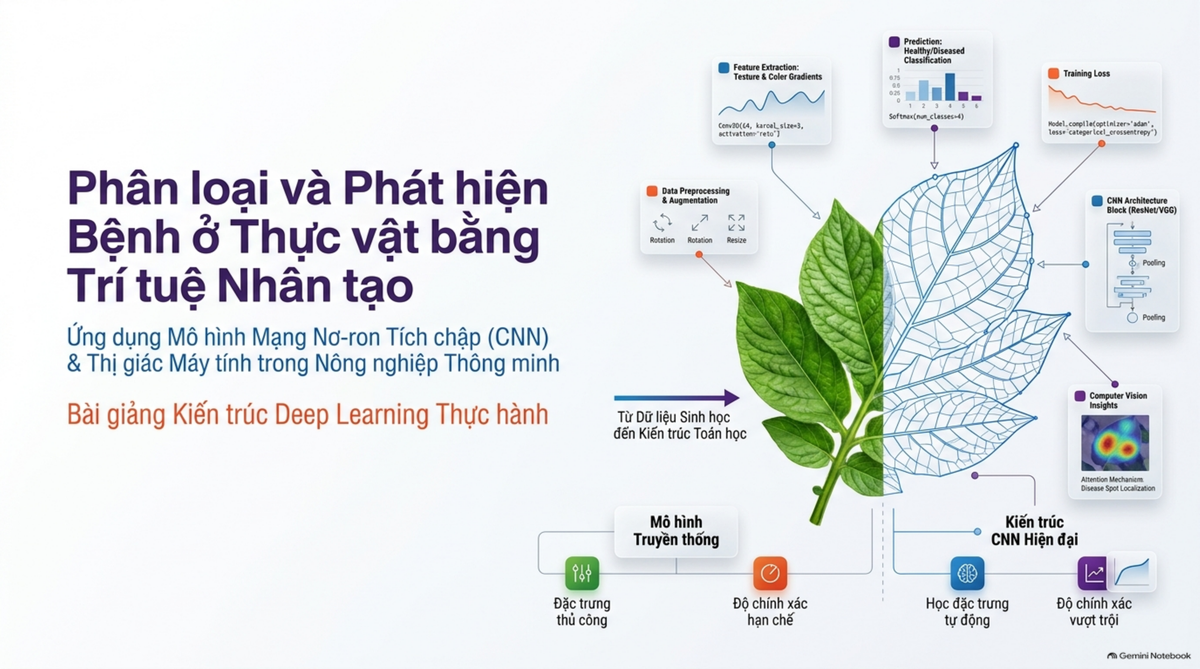
\includegraphics[width=0.9\linewidth,height=0.4\textheight,keepaspectratio]{images_ontap/b3_disease.png}
        \end{column}
    \end{columns}
\end{frame}

% ==========================================
% SLIDE 12: BUỔI 3 - CHẨN ĐOÁN SÂU BỆNH
% ==========================================
\begin{frame}{Buổi 3: Ứng dụng DL trong Nhận diện Sâu bệnh qua hình ảnh}
    \begin{columns}[c]
        \begin{column}{0.55\textwidth}
            \begin{block}{Bài toán thực tế}
                Phát hiện sớm bệnh đạo ôn lúa, bệnh đốm lá táo, cháy lá cà chua, rệp sáp hại sầu riêng từ ảnh chụp bằng điện thoại.
            \end{block}
            \begin{itemize}
                \item \textbf{Tập dữ liệu chuẩn}: PlantVillage (hơn 54,000 ảnh, 38 lớp bệnh cây trồng).
                \item \textbf{Kỹ thuật Data Augmentation}: Xoay góc, lật ngang, điều chỉnh độ sáng, nhiễu Gaussian $\rightarrow$ chống Overfitting khi dữ liệu chụp thực địa biến đổi ánh sáng.
                \item \textbf{Transfer Learning}: Tận dụng trọng số tiền huấn luyện trên ImageNet, chỉ tinh chỉnh (fine-tune) tầng cuối.
            \end{itemize}
        \end{column}
        \begin{column}{0.42\textwidth}
            \centering
            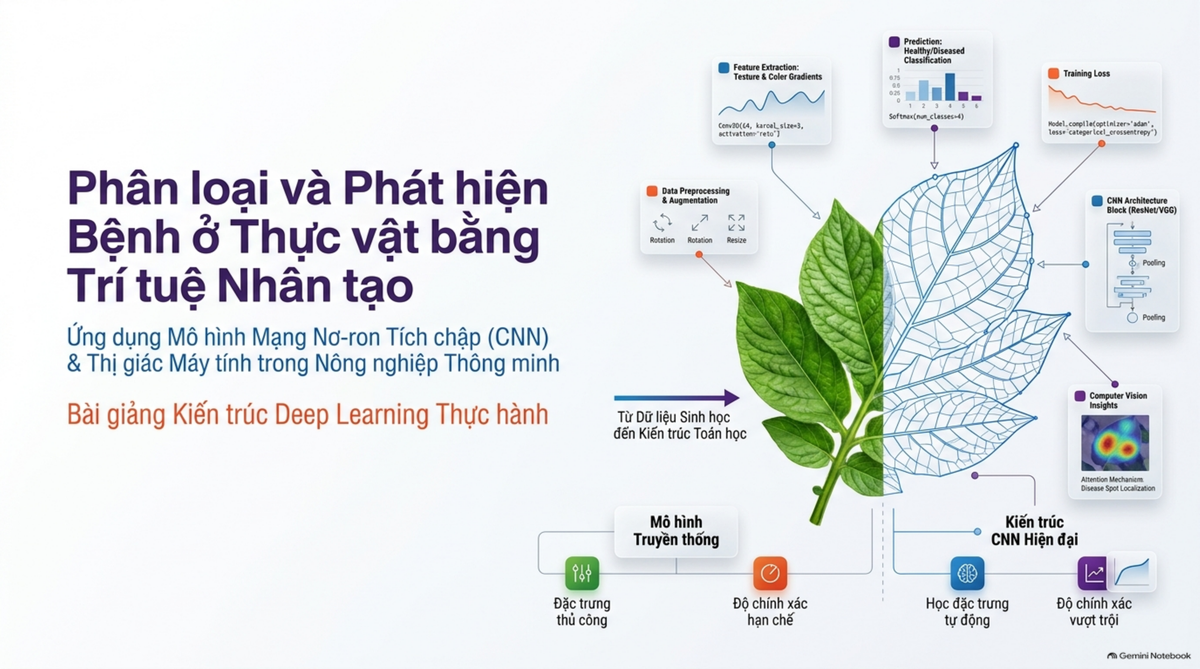
\includegraphics[width=\linewidth,height=0.72\textheight,keepaspectratio]{images_ontap/b3_disease.png}
            \vspace{0.1cm}
            \footnotesize{\textit{Phân loại bệnh học thực vật tự động}}
        \end{column}
    \end{columns}
\end{frame}

% ==========================================
% SLIDE 13: BUỔI 4 - THỊ GIÁC MÁY TÍNH
% ==========================================
\begin{frame}{Buổi 4: Thị giác máy tính (Computer Vision) trong Nông nghiệp}
    \begin{columns}[c]
        \begin{column}{0.55\textwidth}
            \textbf{Từ Xử lý ảnh số (IP) đến Computer Vision (CV):}
            \begin{itemize}
                \item \textbf{Không gian màu}: RGB, HSV, Lab (HSV rất hữu hiệu để tách biệt màu xanh lá cây hoặc màu quả chín khỏi đất).
                \item \textbf{Phân đoạn ảnh (Segmentation)}: Tách nền lá cây, vùng lá bị tổn thương (Otsu Thresholding, Watershed, U-Net).
                \item \textbf{Hình thái học (Morphology)}: Dilation, Erosion để lọc sạn nhiễu camera đồng ruộng.
            \end{itemize}
            \begin{block}{Mục tiêu}
                Cung cấp cho máy tính "đôi mắt" để tự động nhận dạng, đo đếm và phân loại mà không cần con người can thiệp.
            \end{block}
        \end{column}
        \begin{column}{0.42\textwidth}
            \centering
            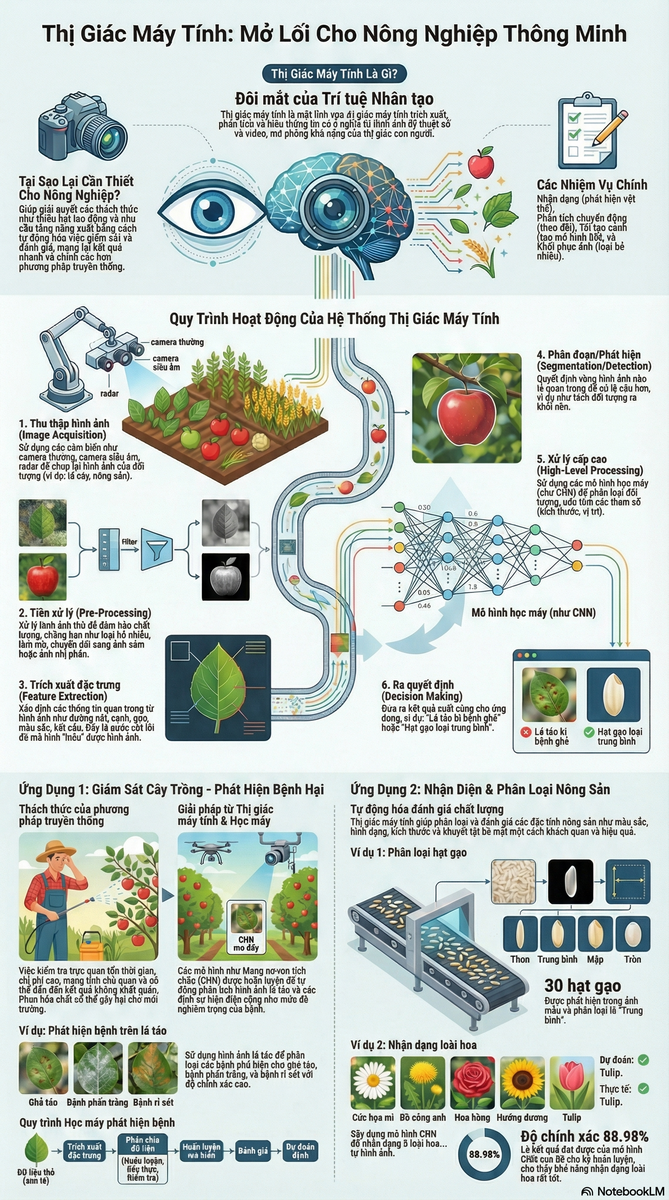
\includegraphics[width=\linewidth,height=0.72\textheight,keepaspectratio]{images_ontap/b4_infographic.png}
        \end{column}
    \end{columns}
\end{frame}

% ==========================================
% SLIDE 14: BUỔI 4 - NHẬN DIỆN LOÀI HOA/CÂY
% ==========================================
\begin{frame}{Buổi 4: Nhận diện Loài hoa \& Phân loại Phẩm cấp Nông sản}
    \begin{columns}[c]
        \begin{column}{0.55\textwidth}
            \begin{block}{Nhận diện loài thực vật (Species Recognition)}
                \begin{itemize}
                    \item Phân biệt các giống hoa, cây dược liệu quý, phân biệt cỏ dại và cây trồng chính.
                    \item Trích xuất đặc trưng hình thái: gân lá, nhụy hoa, cánh hoa.
                \end{itemize}
            \end{block}
            \begin{exampleblock}{Phân loại phẩm cấp quả (Fruit Grading)}
                \begin{itemize}
                    \item Đo kích thước đường kính, độ tròn quả cà chua, cam, táo.
                    \item Đánh giá độ chín qua phổ màu vỏ quả.
                    \item Phát hiện vết trầy xước, dập nát trên băng chuyền tự động.
                \end{itemize}
            \end{exampleblock}
        \end{column}
        \begin{column}{0.42\textwidth}
            \centering
            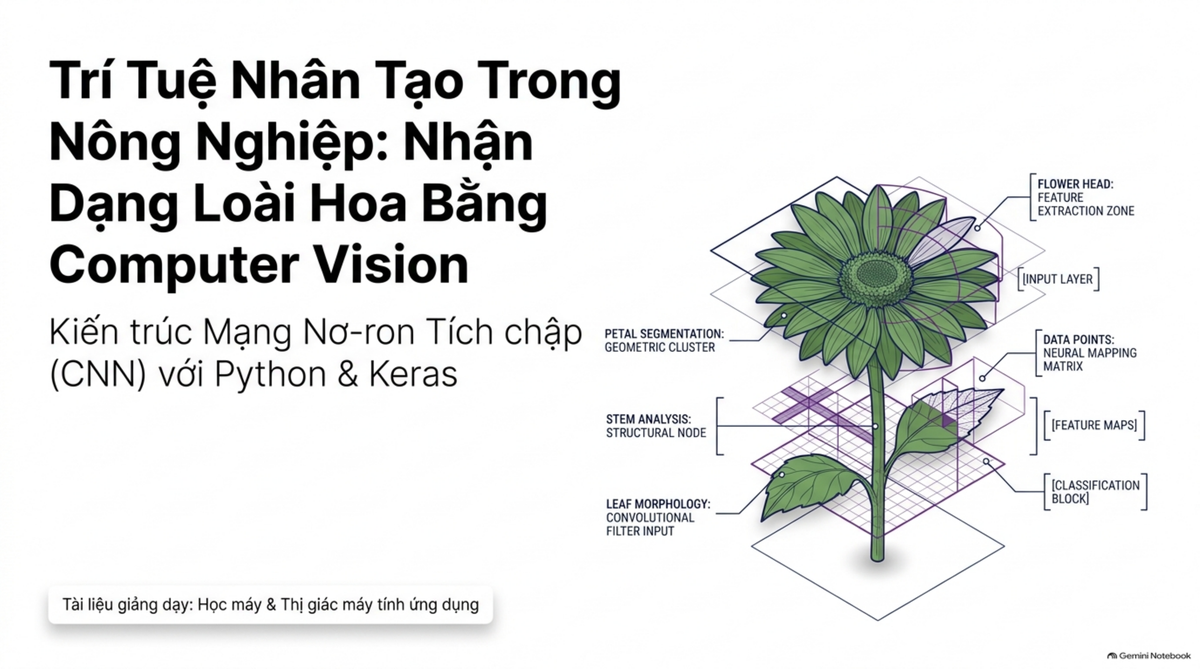
\includegraphics[width=\linewidth,height=0.72\textheight,keepaspectratio]{images_ontap/b4_species.png}
            \vspace{0.1cm}
            \footnotesize{\textit{Hệ thống nhận diện loài hoa và quả}}
        \end{column}
    \end{columns}
\end{frame}

% ==========================================
% SLIDE 15: BUỔI 4 - PHÁT HIỆN ĐỐI TƯỢNG (YOLO)
% ==========================================
\begin{frame}{Buổi 4: Phát hiện Đối tượng (Object Detection) \& Đếm sản lượng}
    \begin{columns}[c]
        \begin{column}{0.55\textwidth}
            \begin{block}{Sự khác biệt: Phân loại vs Phát hiện}
                \begin{itemize}
                    \item \textbf{Classification}: "Ảnh này có quả táo không?"
                    \item \textbf{Object Detection}: "Quả táo ở tọa độ Bounding Box nào $[x, y, w, h]$ và có bao nhiêu quả?"
                \end{itemize}
            \end{block}
            \textbf{Các kiến trúc thời gian thực (Real-time):}
            \begin{itemize}
                \item \textbf{YOLO (You Only Look Once - v5/v8/v11)}: Tốc độ xử lý cực nhanh (30--60 FPS), phù hợp gắn trên Drone hoặc robot thu hoạch.
                \item \textbf{Ứng dụng}: Đếm số lượng hoa bưởi, đếm chùm nho, định vị quả chín cho tay gắp Robot hái quả tự động.
            \end{itemize}
        \end{column}
        \begin{column}{0.42\textwidth}
            \centering
            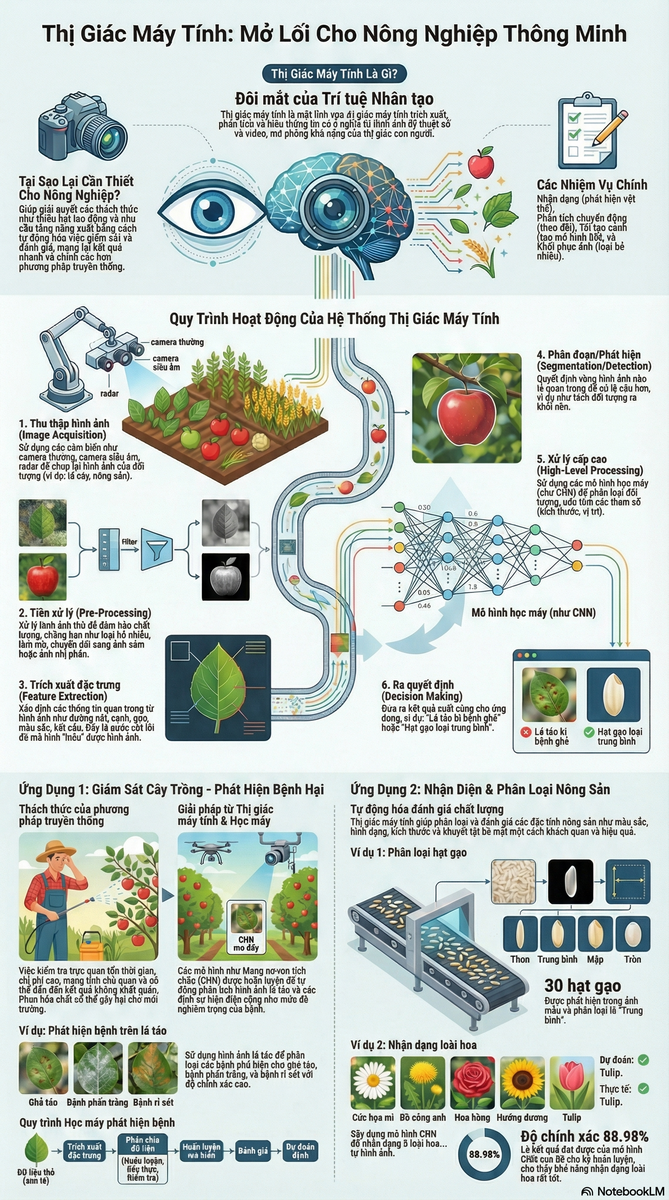
\includegraphics[width=\linewidth,height=0.72\textheight,keepaspectratio]{images_ontap/b4_infographic.png}
        \end{column}
    \end{columns}
\end{frame}

% ==========================================
% SLIDE 16: BUỔI 5 - HỆ CHUYÊN GIA NÔNG NGHIỆP
% ==========================================
\begin{frame}{Buổi 5: Hệ hỗ trợ ra quyết định (DSS) \& Hệ chuyên gia Nông nghiệp}
    \begin{columns}[c]
        \begin{column}{0.55\textwidth}
            \begin{block}{Cấu trúc 3 thành phần của Hệ chuyên gia (Expert System)}
                \begin{enumerate}
                    \item \textbf{Cơ sở tri thức (Knowledge Base)}: Tập hợp tri thức chuyên gia nông học dưới dạng luật \texttt{IF-THEN} và Ontology.
                    \item \textbf{Động cơ suy diễn (Inference Engine)}: Suy diễn tiến (Forward Chaining) từ triệu chứng $\rightarrow$ bệnh; Suy diễn lùi (Backward Chaining).
                    \item \textbf{Giao diện người dùng}: Tiếp nhận thông tin nông hộ và trả lời khuyến nghị.
                \end{enumerate}
            \end{block}
            \begin{alertblock}{Ưu thế vượt trội}
                Giải thích được nguyên nhân (\textit{"Explainable AI"}), nông dân hiểu rõ \textbf{tại sao} cần bón loại phân này.
            \end{alertblock}
        \end{column}
        \begin{column}{0.42\textwidth}
            \centering
            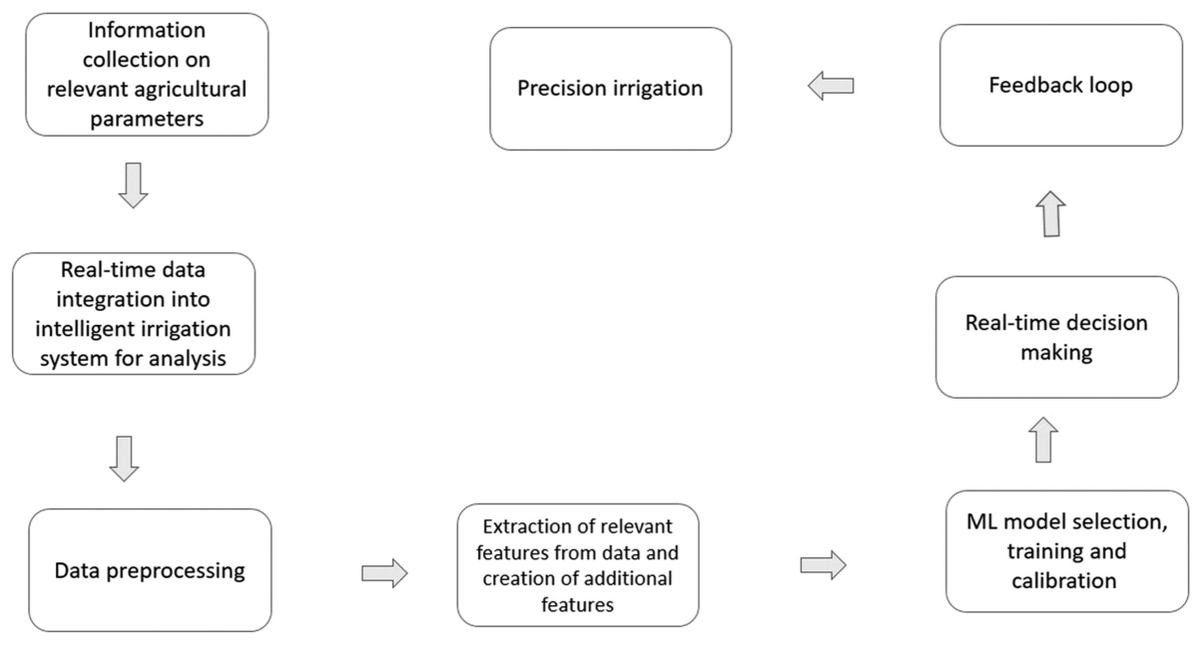
\includegraphics[width=\linewidth,height=0.72\textheight,keepaspectratio]{images_ontap/b5_expert_system.png}
            \vspace{0.1cm}
            \footnotesize{\textit{Sơ đồ luồng suy diễn hệ chuyên gia DSS}}
        \end{column}
    \end{columns}
\end{frame}

% ==========================================
% SLIDE 17: BUỔI 5 - DSS CÂY TRỒNG TÂY NGUYÊN
% ==========================================
\begin{frame}{Buổi 5: Case Studies: Hệ Chuyên gia Cây trồng Tây Nguyên}
    \begin{columns}[c]
        \begin{column}{0.55\textwidth}
            \textbf{Bộ hệ chuyên gia chuẩn hóa xây dựng trong khóa học:}
            \begin{itemize}
                \item \textbf{DSS Cà phê Tây Nguyên}: Chuẩn đoán thiếu vi lượng (Bo, Kẽm), tưới nước siết hoa bung đồng loạt.
                \item \textbf{DSS Bảo vệ Thực vật Hồ tiêu}: Cảnh báo sớm bệnh chết nhanh (\textit{Phytophthora}), chết chậm (\textit{Nematodes}).
                \item \textbf{DSS Sầu riêng}: Quản lý cơi đọt, chặn đọt khi nuôi trái, chống sốc nhiệt rụng bông.
                \item \textbf{DSS Chế biến Fine Robusta}: Kiểm soát thang điểm Cupping SCA, kiểm soát lên men yếm khí.
            \end{itemize}
        \end{column}
        \begin{column}{0.42\textwidth}
            \begin{exampleblock}{Tích hợp công cụ tính toán số}
                \begin{itemize}
                    \item Chuyển đổi N-P-K thực tế sang phân đơn/phân phức.
                    \item Tính toán lượng vôi/thạch cao rửa mặn, khử chua đất đỏ Bazan.
                \end{itemize}
            \end{exampleblock}
            \centering
            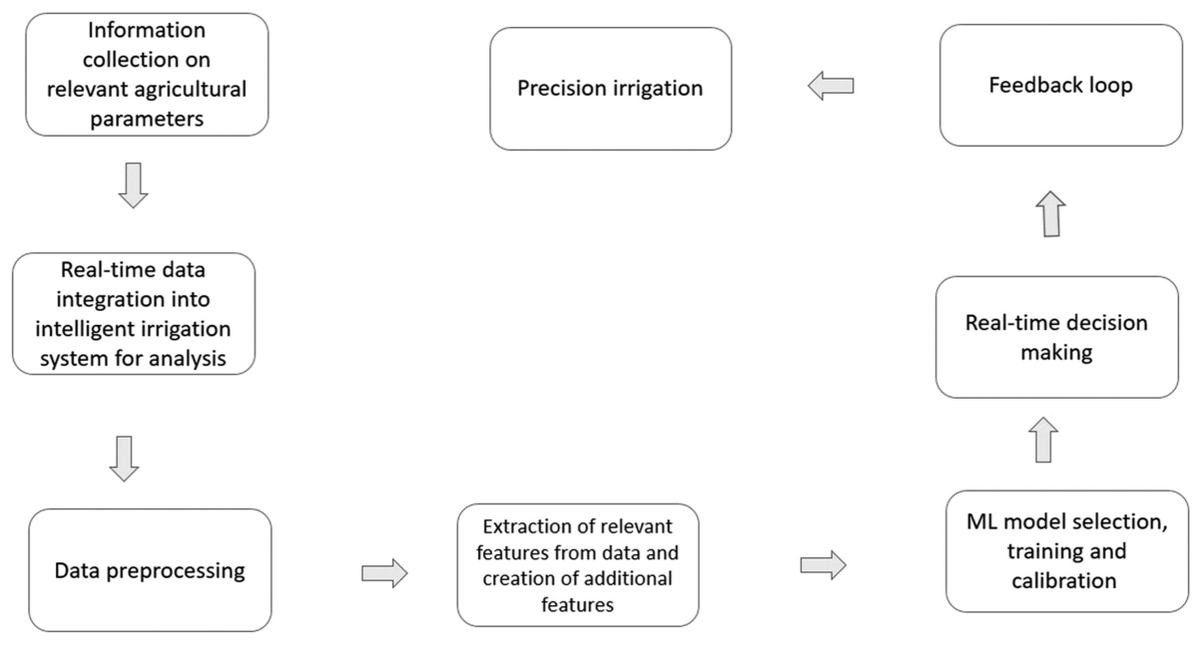
\includegraphics[width=0.85\linewidth,height=0.4\textheight,keepaspectratio]{images_ontap/b5_expert_system.png}
        \end{column}
    \end{columns}
\end{frame}

% ==========================================
% SLIDE 18: BUỔI 5 - TỔNG HỢP ÔN TẬP GIỮA KỲ
% ==========================================
\begin{frame}{Buổi 5: Đánh giá \& Hệ thống hóa kiến thức Giai đoạn 1}
    \begin{columns}[c]
        \begin{column}{0.55\textwidth}
            \begin{block}{Ma trận kiến thức nửa đầu khóa học}
                \begin{itemize}
                    \item \textbf{Tư duy AI}: Hiểu rõ bài toán nông nghiệp nào cần Heuristics/Luật, bài toán nào cần ML bảng, bài toán nào cần DL ảnh.
                    \item \textbf{Metric đánh giá}: Phân biệt Accuracy (dễ bị đánh lừa khi mẫu mất cân bằng) với F1-Score, ROC-AUC, Confusion Matrix.
                    \item \textbf{Thực hành chuẩn}: Tiền xử lý, chống rò rỉ dữ liệu (Data Leakage), phân chia tập kiểm thử độc lập.
                \end{itemize}
            \end{block}
        \end{column}
        \begin{column}{0.42\textwidth}
            \centering
            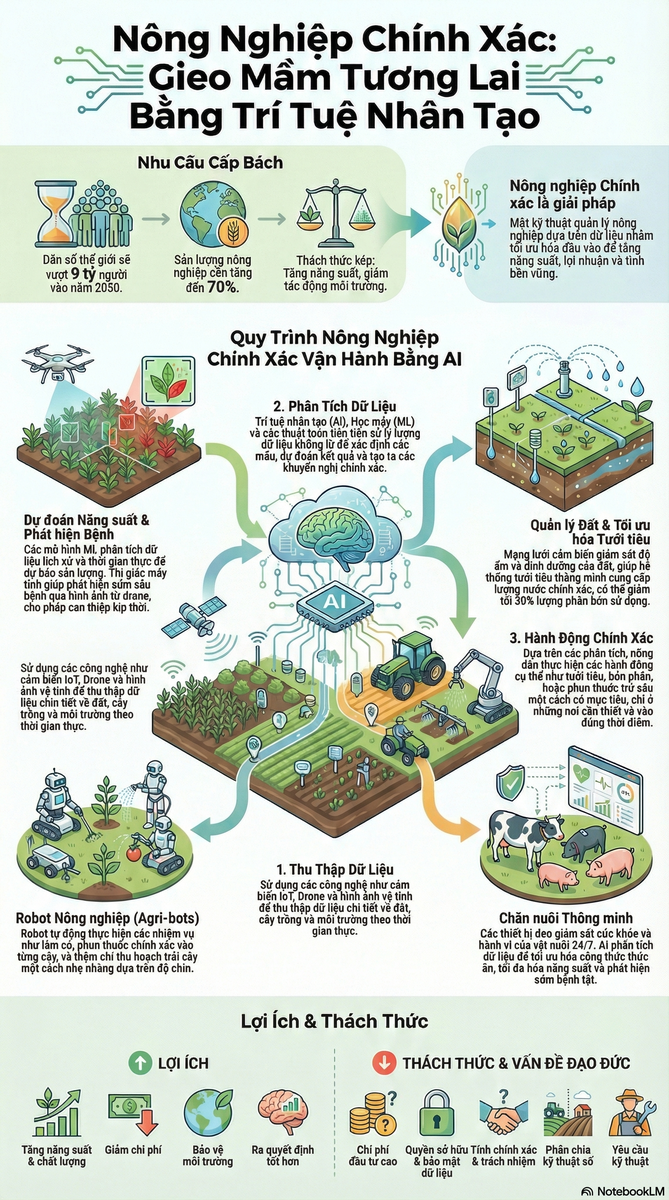
\includegraphics[width=\linewidth,height=0.72\textheight,keepaspectratio]{images_ontap/b1_infographic.png}
            \vspace{0.1cm}
            \footnotesize{\textit{Nền tảng kiểm tra giữa kỳ 100\% thực tiễn}}
        \end{column}
    \end{columns}
\end{frame}

% ==========================================
% SLIDE 19: BUỔI 6 - QUẢN LÝ NƯỚC & IOT
% ==========================================
\begin{frame}{Buổi 6: IoT \& Mạng lưới Cảm biến Nông nghiệp Thông minh}
    \begin{columns}[c]
        \begin{column}{0.55\textwidth}
            \begin{block}{Hạ tầng thu thập dữ liệu tự động}
                \begin{itemize}
                    \item \textbf{Cảm biến đất}: Độ ẩm thể tích (VWC), Độ dẫn điện EC, pH, N-P-K, nhiệt độ đất.
                    \item \textbf{Trạm thời tiết vi mô (AWS)}: Bức xạ mặt trời, tốc độ gió, vũ lượng, độ ẩm không khí.
                    \item \textbf{Giao thức truyền thông}: LoRaWAN (truyền xa 5--15km, tiết kiệm pin), Zigbee, 4G/NB-IoT.
                \end{itemize}
            \end{block}
            \begin{alertblock}{Bài toán cốt lõi}
                Đưa dữ liệu cảm biến thời gian thực về Cloud/Edge để AI ra quyết định điều khiển van tưới tự động.
            \end{alertblock}
        \end{column}
        \begin{column}{0.42\textwidth}
            \centering
            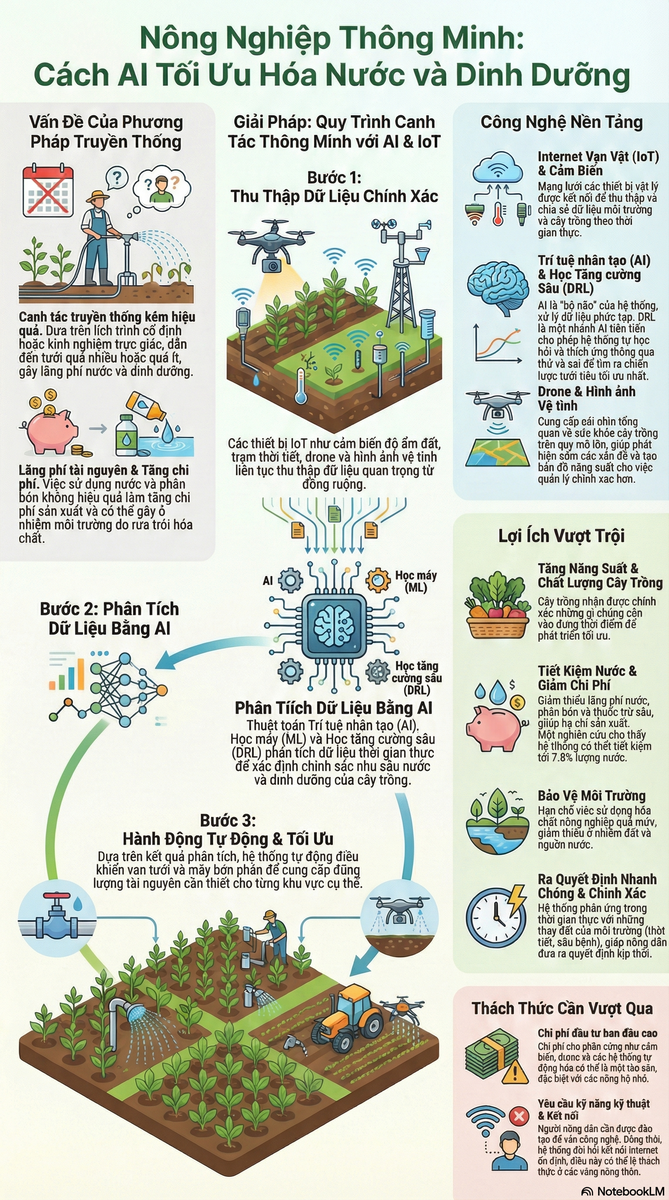
\includegraphics[width=\linewidth,height=0.72\textheight,keepaspectratio]{images_ontap/b6_infographic.png}
        \end{column}
    \end{columns}
\end{frame}

% ==========================================
% SLIDE 20: BUỔI 6 - TƯỚI TIÊU THÔNG MINH (DRL)
% ==========================================
\begin{frame}{Buổi 6: Tưới tiêu Thông minh \& Học tăng cường sâu (DRL)}
    \begin{columns}[c]
        \begin{column}{0.55\textwidth}
            \begin{block}{Hạn chế của tưới tiêu theo hẹn giờ truyền thống}
                Tưới cố định gây ngập úng vào ngày mưa hoặc thiếu nước khi trời nắng gắt $\rightarrow$ lãng phí 30--50\% nước.
            \end{block}
            \textbf{Mô hình DRL (Deep Reinforcement Learning):}
            \begin{itemize}
                \item \textbf{Trạng thái ($S$)}: Độ ẩm đất hiện tại + Dự báo thời tiết 24h tới + Giai đoạn sinh trưởng.
                \item \textbf{Hành động ($A$)}: Bật/tắt bơm, thời gian tưới $t$ phút.
                \item \textbf{Hàm thưởng ($R$)}: Duy trì độ ẩm trong ngưỡng tối ưu + Phạt khi tiêu hao điện/nước quá mức.
            \end{itemize}
        \end{column}
        \begin{column}{0.42\textwidth}
            \centering
            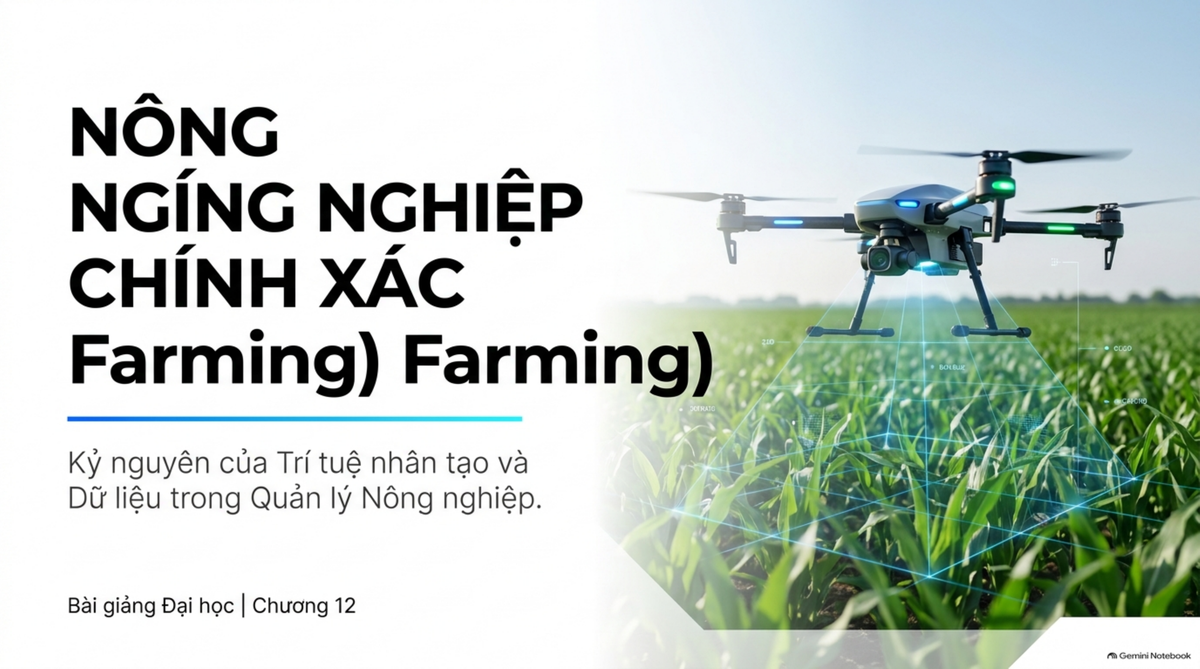
\includegraphics[width=\linewidth,height=0.72\textheight,keepaspectratio]{images_ontap/b6_smart_irrigation.png}
            \vspace{0.1cm}
            \footnotesize{\textit{Hệ thống tưới tự thích ứng theo nhu cầu cây trồng}}
        \end{column}
    \end{columns}
\end{frame}

% ==========================================
% SLIDE 21: BUỔI 6 - QUẢN LÝ DINH DƯỠNG (FERTIGATION)
% ==========================================
\begin{frame}{Buổi 6: Quản lý Dinh dưỡng \& Tối ưu hóa Phân bón}
    \begin{columns}[c]
        \begin{column}{0.55\textwidth}
            \begin{block}{Precision Fertigation (Tưới phân chính xác)}
                Châm phân tự động hòa tan theo hệ thống tưới nhỏ giọt, điều khiển tự động bằng thuật toán AI.
            \end{block}
            \begin{itemize}
                \item \textbf{Cân bằng ion trong đất}: Tránh hiện tượng tích tụ muối làm chai đất, cháy rễ do thừa phân hóa học.
                \item \textbf{Tối ưu hóa đa mục tiêu}: Cực đại hóa năng suất cây trồng nhưng Cực tiểu hóa chi phí phân bón và tồn dư Nitrat trong đất/nước ngầm.
                \item Thuật toán di truyền (Genetic Algorithm) và Gradient Descent tìm tỷ lệ phối trộn $N:P:K$ lý tưởng theo tuần tuổi.
            \end{itemize}
        \end{column}
        \begin{column}{0.42\textwidth}
            \centering
            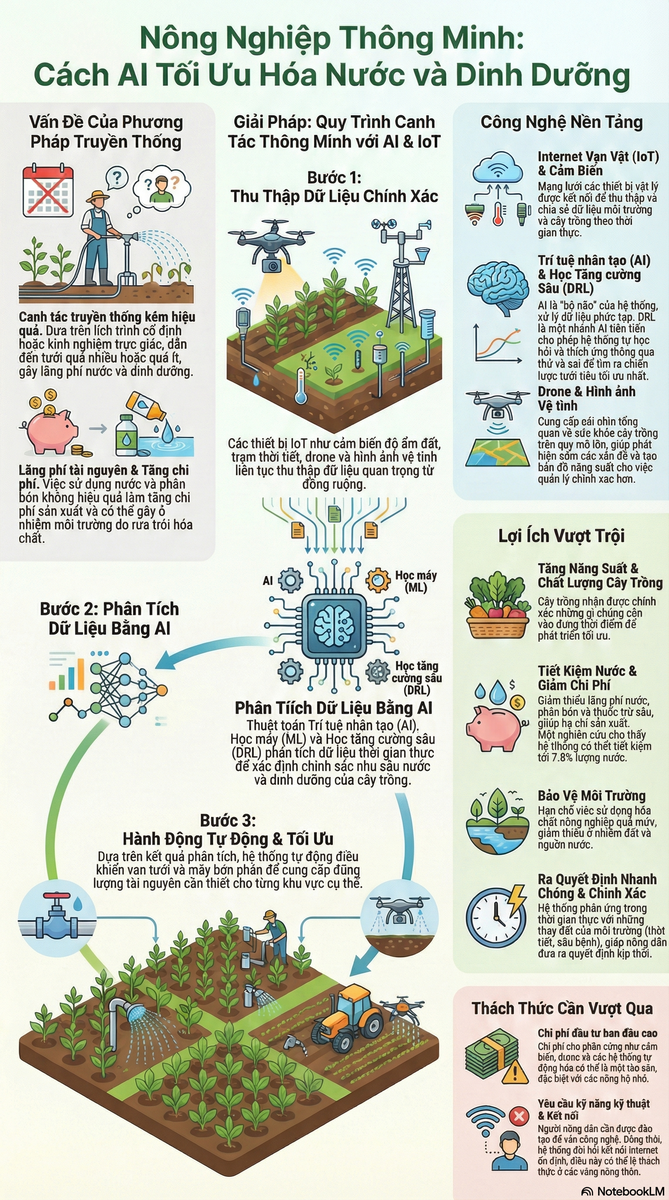
\includegraphics[width=\linewidth,height=0.72\textheight,keepaspectratio]{images_ontap/b6_infographic.png}
        \end{column}
    \end{columns}
\end{frame}

% ==========================================
% SLIDE 22: BUỔI 7 - DỮ LIỆU LỚN & VIỄN THÁM
% ==========================================
\begin{frame}{Buổi 7: Dữ liệu lớn \& Viễn thám Nông nghiệp (NDVI/Satellite)}
    \begin{columns}[c]
        \begin{column}{0.55\textwidth}
            \begin{block}{Viễn thám quang phổ (Remote Sensing)}
                Ảnh vệ tinh (Sentinel-2, Landsat) và Camera đa phổ gắn trên Drone/Máy bay không người lái.
            \end{block}
            \textbf{Chỉ số thực vật NDVI (Normalized Difference Vegetation Index):}
            \[ \text{NDVI} = \frac{\text{NIR} - \text{RED}}{\text{NIR} + \text{RED}} \]
            \begin{itemize}
                \item \textbf{NIR}: Cận hồng ngoại (lá khỏe phản xạ mạnh).
                \item \textbf{RED}: Ánh sáng đỏ (diệp lục hấp thụ để quang hợp).
                \item $\text{NDVI} > 0.6$: Thảm thực vật xanh tốt, sinh khối khỏe mạnh; $\text{NDVI} < 0.2$: Đất trống, cây suy thoái/héo úa.
            \end{itemize}
        \end{column}
        \begin{column}{0.42\textwidth}
            \centering
            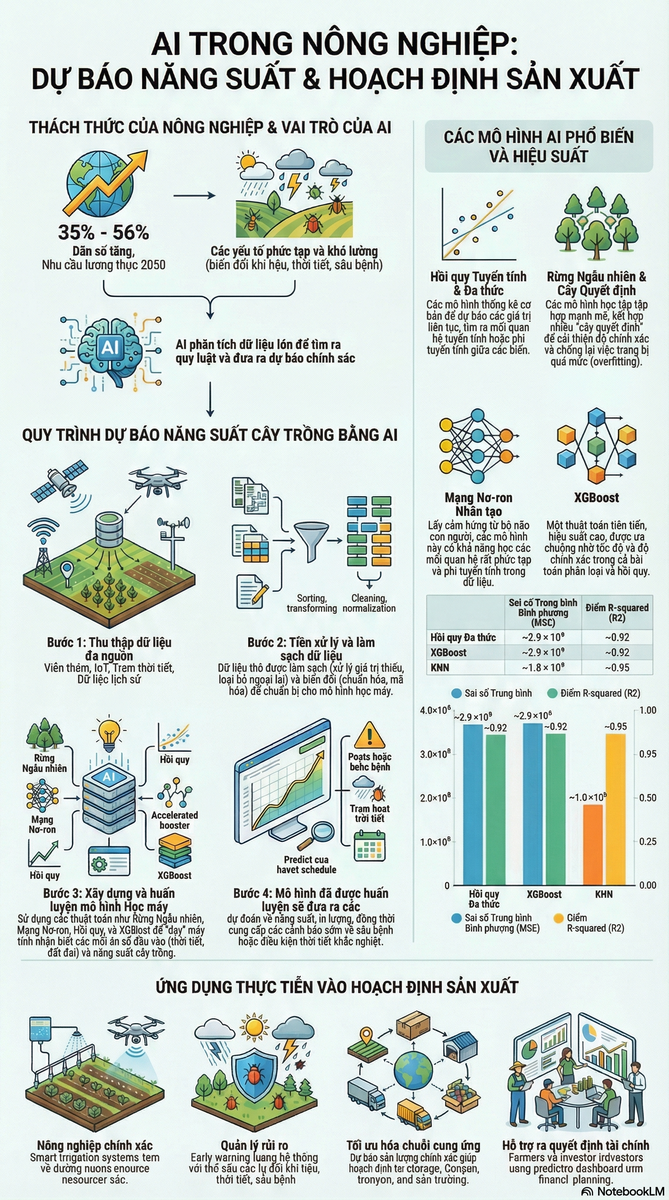
\includegraphics[width=\linewidth,height=0.72\textheight,keepaspectratio]{images_ontap/b7_infographic.png}
        \end{column}
    \end{columns}
\end{frame}

% ==========================================
% SLIDE 23: BUỔI 7 - DỰ BÁO NĂNG SUẤT
% ==========================================
\begin{frame}{Buổi 7: Mô hình Dự báo Năng suất Cây trồng (Crop Yield)}
    \begin{columns}[c]
        \begin{column}{0.55\textwidth}
            \begin{block}{Thách thức của bài toán dự báo}
                Năng suất phụ thuộc vào hàm phi tuyến đa biến: giống cây, thổ nhưỡng, thời tiết lũy kế và kỹ thuật chăm sóc.
            \end{block}
            \textbf{Kiến trúc mô hình hiện đại kết hợp:}
            \begin{itemize}
                \item \textbf{CNN 2D/3D}: Trích xuất đặc trưng không gian từ bản đồ chuỗi ảnh viễn thám NDVI/EVI.
                \item \textbf{LSTM / GRU / Transformer}: Nắm bắt chuỗi phụ thuộc thời gian của lượng mưa, nhiệt độ tích lũy (GDD).
                \item \textbf{XGBoost / LightGBM}: Mô hình nền vững chắc khi kết hợp các bảng số liệu nông học truyền thống.
            \end{itemize}
        \end{column}
        \begin{column}{0.42\textwidth}
            \centering
            
\includegraphics[width=\linewidth,height=0.72\textheight,keepaspectratio]{images_ontap/b7_crop_yield.png}
            \vspace{0.1cm}
            \footnotesize{\textit{Dự báo năng suất phục vụ bảo hiểm nông nghiệp}}
        \end{column}
    \end{columns}
\end{frame}

% ==========================================
% SLIDE 24: BUỔI 7 - HOẠCH ĐỊNH CHUỖI CUNG ỨNG
% ==========================================
\begin{frame}{Buổi 7: Hoạch định Sản xuất \& Quản trị Chuỗi cung ứng Nông sản}
    \begin{columns}[c]
        \begin{column}{0.55\textwidth}
            \begin{block}{Giá trị kinh tế của AI dự báo}
                \begin{itemize}
                    \item \textbf{Tránh khủng hoảng thừa}: Dự báo trước sản lượng toàn vùng giúp cơ quan quản lý điều tiết mùa vụ, tránh cảnh \textit{"được mùa mất giá"}.
                    \item \textbf{Lập kế hoạch logistics}: Dự báo chính xác ngày thu hoạch để điều động xe tải lạnh, nhân công thu hái, kho bảo quản.
                    \item \textbf{Hợp đồng bao tiêu}: Giúp hợp tác xã và doanh nghiệp chế biến ký kết hợp đồng xuất khẩu sớm.
                \end{itemize}
            \end{block}
        \end{column}
        \begin{column}{0.42\textwidth}
            \centering
            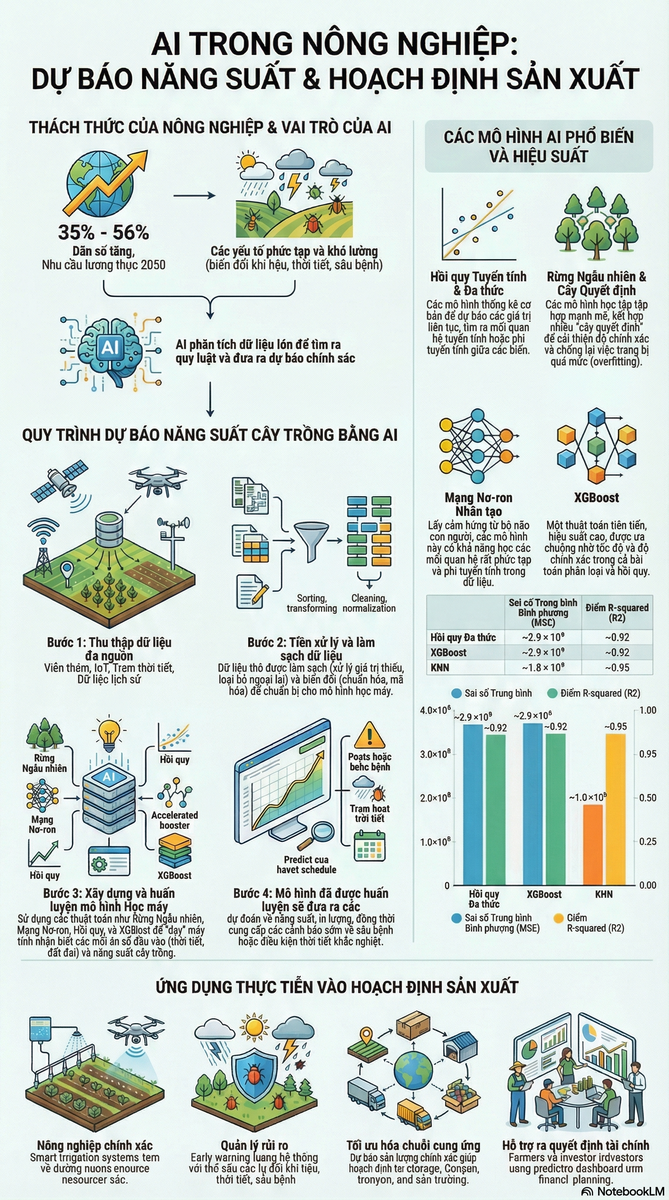
\includegraphics[width=\linewidth,height=0.72\textheight,keepaspectratio]{images_ontap/b7_infographic.png}
        \end{column}
    \end{columns}
\end{frame}

% ==========================================
% SLIDE 25: BUỔI 8 - CHECKLIST DỰ ÁN ML
% ==========================================
\begin{frame}{Buổi 8: Machine Learning Project Checklist chuẩn quốc tế}
    \begin{columns}[c]
        \begin{column}{0.55\textwidth}
            \begin{block}{Quy trình 8 bước theo Géron (Hands-on ML)}
                \begin{enumerate}
                    \item Định hình bài toán \& Mục tiêu kinh doanh.
                    \item Thu thập dữ liệu \& Khảo sát thực địa.
                    \item Khám phá trực quan hóa dữ liệu (EDA).
                    \item Chuẩn bị dữ liệu cho thuật toán ML.
                    \item Lựa chọn danh sách ngắn các mô hình triển vọng.
                    \item Tinh chỉnh siêu tham số (Fine-tune, GridSearch).
                    \item Thuyết trình giải pháp \& Đo lường hiệu quả.
                    \item Triển khai, giám sát (Monitoring) \& Bảo trì hệ thống.
                \end{enumerate}
            \end{block}
        \end{column}
        \begin{column}{0.42\textwidth}
            \centering
            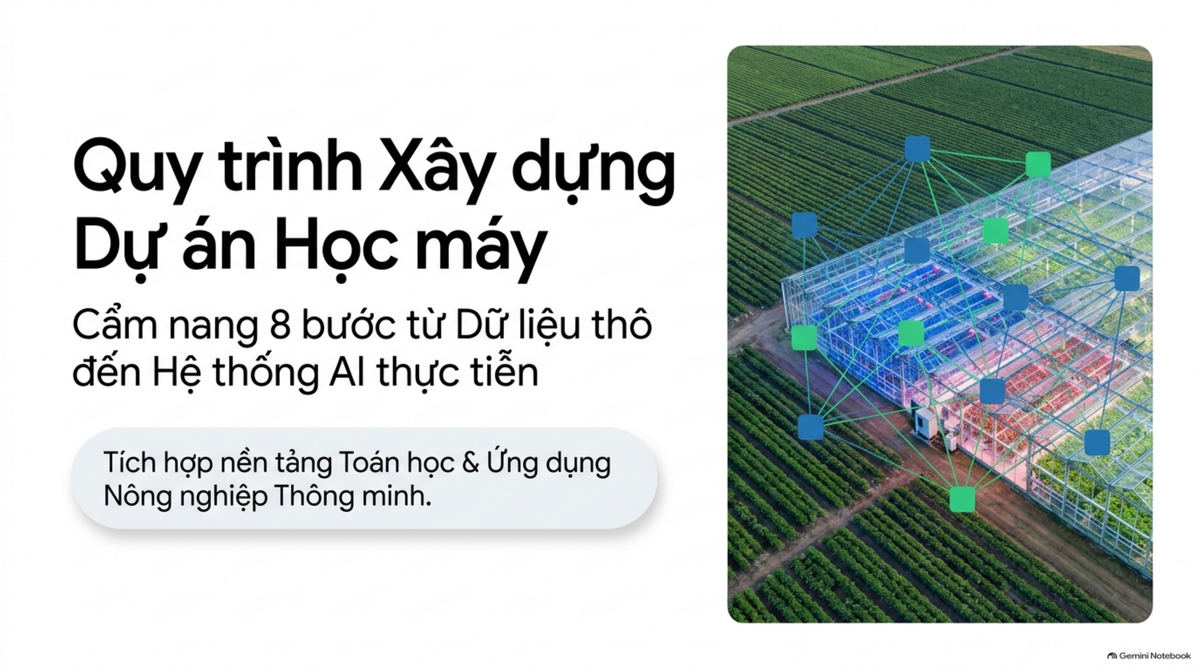
\includegraphics[width=\linewidth,height=0.72\textheight,keepaspectratio]{images_ontap/b8_checklist.png}
            \vspace{0.1cm}
            \footnotesize{\textit{Checklist kỹ thuật quản lý dự án AI}}
        \end{column}
    \end{columns}
\end{frame}

% ==========================================
% SLIDE 26: BUỔI 8 - ĐÁNH GIÁ DỰ ÁN NHÓM
% ==========================================
\begin{frame}{Buổi 8: Báo cáo Dự án Nhóm \& Đạo đức Dữ liệu Nông hộ}
    \begin{columns}[c]
        \begin{column}{0.55\textwidth}
            \begin{block}{Bài học từ các dự án sinh viên}
                \begin{itemize}
                    \item \textbf{Bẫy Overfitting}: Độ chính xác trên tập Train 99\% nhưng ra đồng ruộng chụp ảnh thực tế chỉ còn 60\% do bóng râm, bụi bẩn ống kính.
                    \item \textbf{Tầm quan trọng của Domain Knowledge}: Kỹ sư AI bắt buộc phải tham vấn chuyên gia nông học để hiểu chu kỳ bệnh.
                \end{itemize}
            \end{block}
            \begin{alertblock}{Bảo vệ quyền lợi nông dân}
                Không độc quyền dữ liệu, bảo mật vị trí tọa độ địa lý vùng trồng, tôn trọng tri thức bản địa.
            \end{alertblock}
        \end{column}
        \begin{column}{0.42\textwidth}
            \centering
            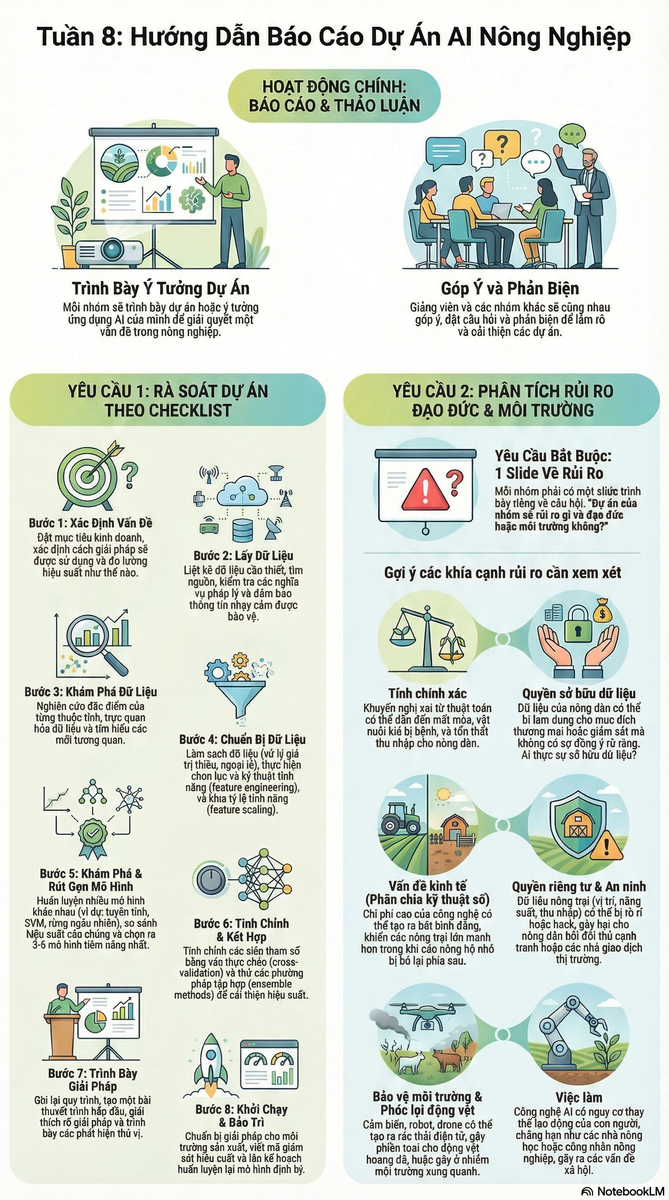
\includegraphics[width=\linewidth,height=0.72\textheight,keepaspectratio]{images_ontap/b8_infographic.png}
        \end{column}
    \end{columns}
\end{frame}

% ==========================================
% SLIDE 27: BUỔI 9 - HỆ SINH THÁI CÔNG CỤ AI
% ==========================================
\begin{frame}{Buổi 9: Hệ sinh thái Công cụ \& Thư viện Lập trình AI}
    \begin{columns}[c]
        \begin{column}{0.55\textwidth}
            \textbf{Tech Stack tiêu chuẩn cho Kỹ sư AI Nông nghiệp:}
            \begin{itemize}
                \item \textbf{Ngôn ngữ lập trình}: Python (3.10+), C++ (cho embedded robot).
                \item \textbf{Khoa học Dữ liệu}: NumPy, Pandas, Scipy, Matplotlib, Seaborn.
                \item \textbf{Machine Learning}: Scikit-learn, XGBoost, LightGBM.
                \item \textbf{Computer Vision}: OpenCV, Albumentations (tăng cường ảnh mạnh mẽ), PIL.
                \item \textbf{Deep Learning Frameworks}: TensorFlow / Keras, PyTorch, Ultralytics YOLOv8.
                \item \textbf{Môi trường}: Google Colab GPU, Jupyter Lab, VS Code.
            \end{itemize}
        \end{column}
        \begin{column}{0.42\textwidth}
            \centering
            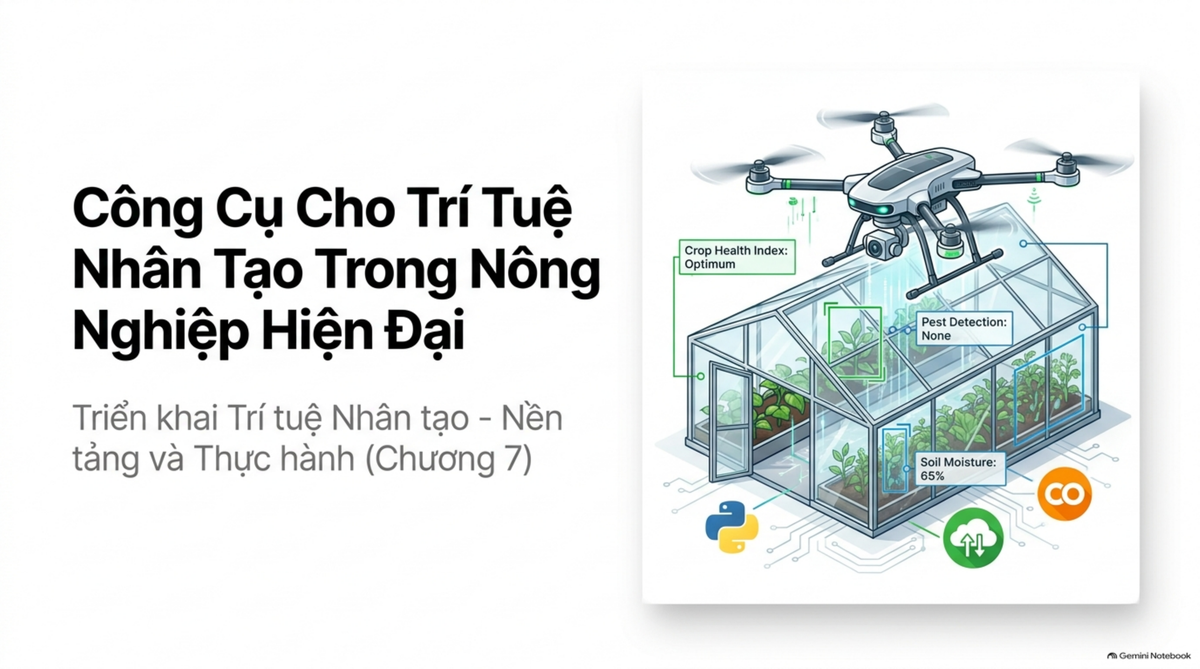
\includegraphics[width=\linewidth,height=0.72\textheight,keepaspectratio]{images_ontap/b9_tools.png}
            \vspace{0.1cm}
            \footnotesize{\textit{Hệ công cụ phần mềm mã nguồn mở}}
        \end{column}
    \end{columns}
\end{frame}

% ==========================================
% SLIDE 28: BUỔI 9 - TIỀN XỬ LÝ & GÁN NHÃN DỮ LIỆU
% ==========================================
\begin{frame}{Buổi 9: Quy trình Thu thập, Làm sạch \& Gán nhãn Dữ liệu}
    \begin{columns}[c]
        \begin{column}{0.55\textwidth}
            \begin{block}{Quy tắc vàng: "Garbage In, Garbage Out"}
                Mô hình dù phức tạp đến đâu cũng thất bại nếu chất lượng dữ liệu đầu vào kém hoặc gán nhãn sai.
            \end{block}
            \textbf{Quy trình chuẩn bị Dataset thực chiến:}
            \begin{enumerate}
                \item \textbf{Chụp ảnh mẫu}: Đa dạng góc chụp, điều kiện ánh sáng (sáng sớm, trưa nắng gắt, chiều tối, sau mưa).
                \item \textbf{Gán nhãn chuyên nghiệp}: Sử dụng Roboflow / LabelImg / CVAT. Gán chuẩn Bounding Box sát viền vết bệnh.
                \item \textbf{Kiểm định chéo}: Nông học kiểm tra lại tính chính xác của nhãn bệnh.
            \end{enumerate}
        \end{column}
        \begin{column}{0.42\textwidth}
            \centering
            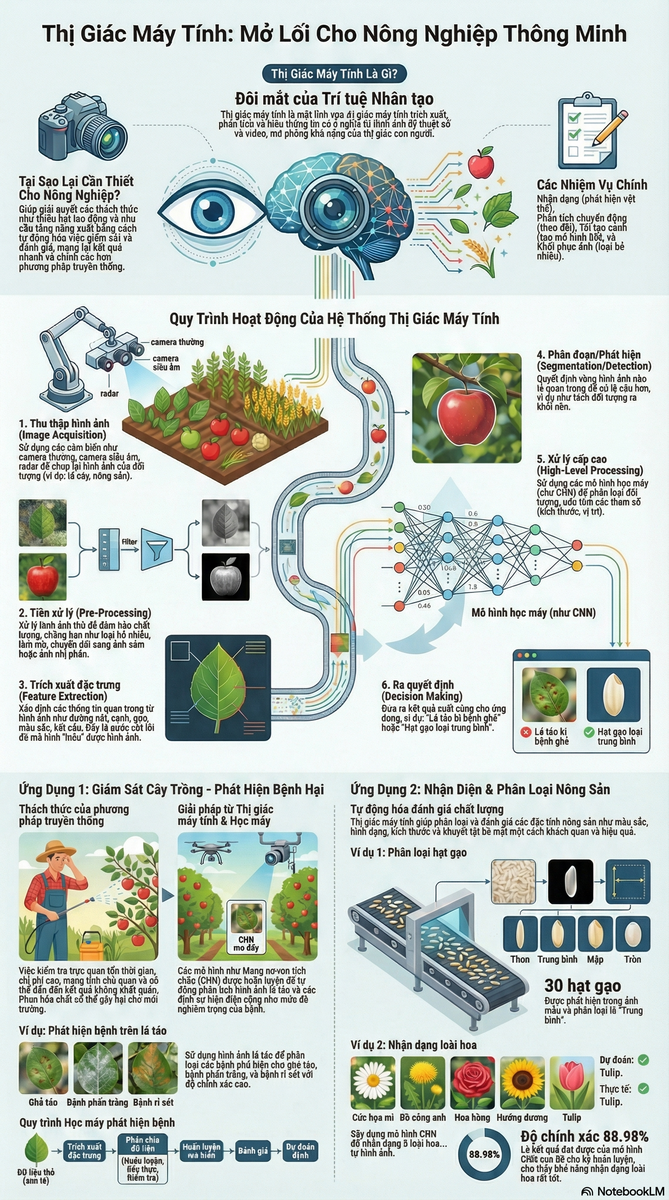
\includegraphics[width=\linewidth,height=0.72\textheight,keepaspectratio]{images_ontap/b4_infographic.png}
        \end{column}
    \end{columns}
\end{frame}

% ==========================================
% SLIDE 29: BUỔI 10 - THỰC HÀNH HUẤN LUYỆN
% ==========================================
\begin{frame}{Buổi 10: Huấn luyện Mô hình Thực chiến \& Tối ưu hóa}
    \begin{columns}[c]
        \begin{column}{0.55\textwidth}
            \begin{block}{Chiến lược huấn luyện hiệu quả}
                \begin{itemize}
                    \item \textbf{Learning Rate Schedule}: Sử dụng Cosine Annealing hoặc ReduceLROnPlateau.
                    \item \textbf{Early Stopping}: Dừng sớm khi Validation Loss không giảm sau 10--15 epochs để tránh Overfitting.
                    \item \textbf{Regularization}: Dropout (0.2--0.5), Batch Normalization, L2 Weight Decay.
                \end{itemize}
            \end{block}
            \begin{exampleblock}{Đánh giá toàn diện}
                Báo cáo Confusion Matrix, phân tích cụ thể các lớp bệnh hay bị nhận diện nhầm lẫn để bổ sung dữ liệu huấn luyện.
            \end{exampleblock}
        \end{column}
        \begin{column}{0.42\textwidth}
            \centering
            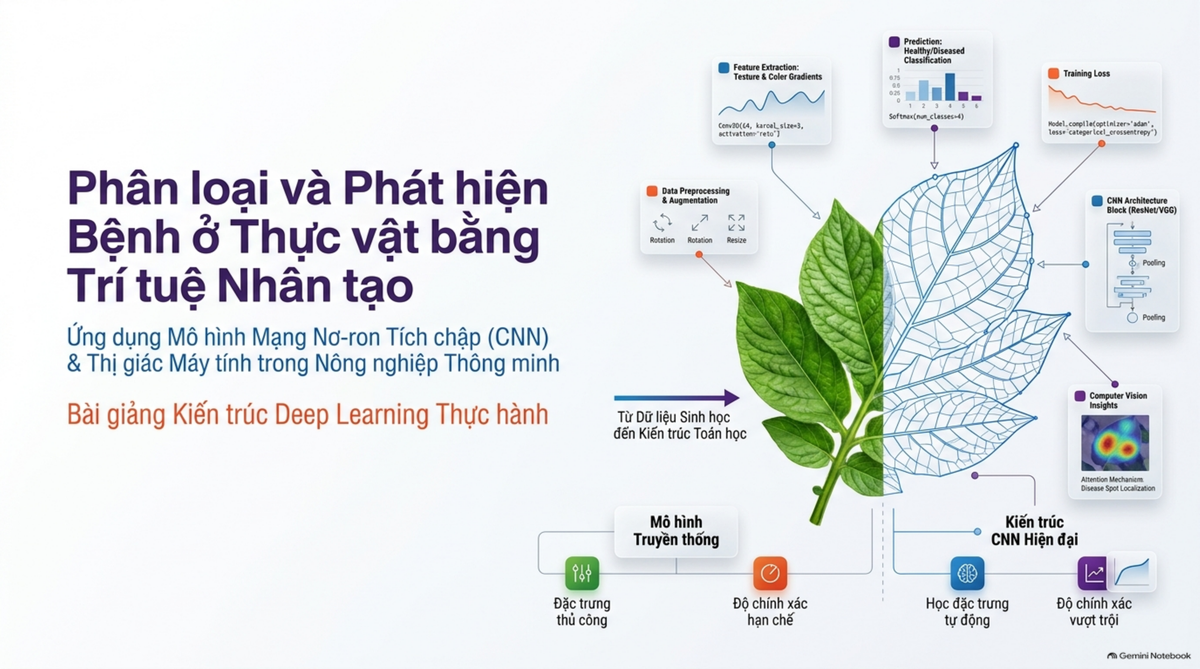
\includegraphics[width=\linewidth,height=0.72\textheight,keepaspectratio]{images_ontap/b3_disease.png}
        \end{column}
    \end{columns}
\end{frame}

% ==========================================
% SLIDE 30: BUỔI 10 - TRIỂN KHAI THIẾT BỊ BIÊN (EDGE AI)
% ==========================================
\begin{frame}{Buổi 10: Triển khai AI trên Thiết bị Biên (Edge AI \& Drone)}
    \begin{columns}[c]
        \begin{column}{0.55\textwidth}
            \begin{block}{Tại sao trang trại cần Edge AI?}
                \begin{itemize}
                    \item Vùng nông thôn, rừng núi thường mất sóng 4G/Internet hoặc băng thông chập chờn.
                    \item Cần phản hồi tức thì (Real-time latency $< 50$ms) cho vòi phun thuốc ngắt tự động khi phát hiện cỏ dại.
                \end{itemize}
            \end{block}
            \textbf{Kỹ thuật nén mô hình:}
            \begin{itemize}
                \item \textbf{Quantization}: Chuyển đổi trọng số từ Float32 $\rightarrow$ INT8 (giảm 75\% dung lượng, tăng tốc 3--4 lần).
                \item \textbf{Định dạng xuất}: ONNX, TensorRT, TensorFlow Lite.
                \item \textbf{Phần cứng}: Raspberry Pi 4/5, NVIDIA Jetson Nano/Orin, ESP32-CAM.
            \end{itemize}
        \end{column}
        \begin{column}{0.42\textwidth}
            \centering
            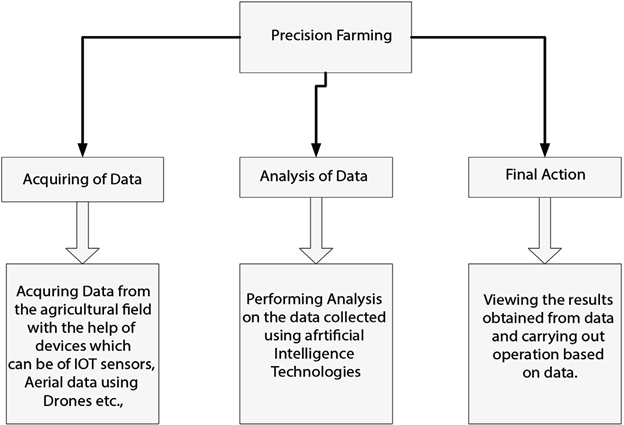
\includegraphics[width=\linewidth,height=0.72\textheight,keepaspectratio]{images_ontap/b10_edgeai.png}
            \vspace{0.1cm}
            \footnotesize{\textit{Thiết bị biên và nông nghiệp chính xác}}
        \end{column}
    \end{columns}
\end{frame}

% ==========================================
% SLIDE 31: TỔNG KẾT BỨC TRANH TOÀN CẢNH
% ==========================================
\begin{frame}{Tổng kết: Nông nghiệp Thông minh từ Truyền thống đến Tự trị}
    \begin{table}[h]
        \centering
        \footnotesize
        \begin{tabular}{p{3.2cm} p{4.5cm} p{5.5cm}}
            \toprule
            \textbf{Giai đoạn} & \textbf{Đặc điểm phương thức} & \textbf{Công nghệ cốt lõi} \\
            \midrule
            \textbf{Nông nghiệp 1.0} & Lao động thủ công, sức kéo gia súc & Nông cụ thô sơ \\
            \textbf{Nông nghiệp 2.0} & Cơ giới hóa, máy kéo, phân hóa học & Động cơ đốt trong, phân NPK \\
            \textbf{Nông nghiệp 3.0} & Tự động hóa, thủy canh, nhà kính & PLC, Hẹn giờ tưới, Cảm biến đơn \\
            \rowcolor{AgriPrimary!15}
            \textbf{Nông nghiệp 4.0 (Hiện nay)} & \textbf{Canh tác số dựa trên dữ liệu} & \textbf{IoT, AI, Computer Vision, Big Data} \\
            \rowcolor{AgriAccent!20}
            \textbf{Nông nghiệp 5.0 (Tương lai)} & \textbf{Tự trị hoàn toàn (Autonomous)} & \textbf{Swarm Robots, DRL, AI Agent, Edge AI} \\
            \bottomrule
        \end{tabular}
    \end{table}
    \vspace{0.2cm}
    \begin{center}
        \textit{"AI không thay thế người nông dân, nhưng người nông dân ứng dụng AI sẽ thay thế người không dùng AI!"}
    \end{center}
\end{frame}

% ==========================================
% SLIDE 32: HƯỚNG DẪN ÔN THI & TÀI NGUYÊN
% ==========================================
\begin{frame}{Tài nguyên Học tập \& Hướng dẫn Ôn thi Cuối kỳ}
    \begin{columns}[c]
        \begin{column}{0.55\textwidth}
            \begin{block}{Cổng thông tin môn học số hóa 100\%}
                \begin{itemize}
                    \item \textbf{Website Môn học}: \url{https://tranthanhthangbmt.github.io/AIAgriculture2026/}
                    \item \textbf{Ngân hàng trắc nghiệm}: 785 câu hỏi tương tác chia theo từng buổi học.
                    \item \textbf{Slide \& Ebook}: 56 Slide PDF và 11 chương giáo trình chuyên khảo song ngữ.
                    \item \textbf{Hỏi đáp Gia sư AI}: Tích hợp NotebookLM giải đáp 24/7 toàn bộ tài liệu môn học.
                \end{itemize}
            \end{block}
            \vspace{0.1cm}
            \centering
            \Large{\textbf{CHÚC CÁC BẠN SINH VIÊN ÔN TẬP TỐT \& ĐẠT KẾT QUẢ CAO!}}
        \end{column}
        \begin{column}{0.42\textwidth}
            \centering
            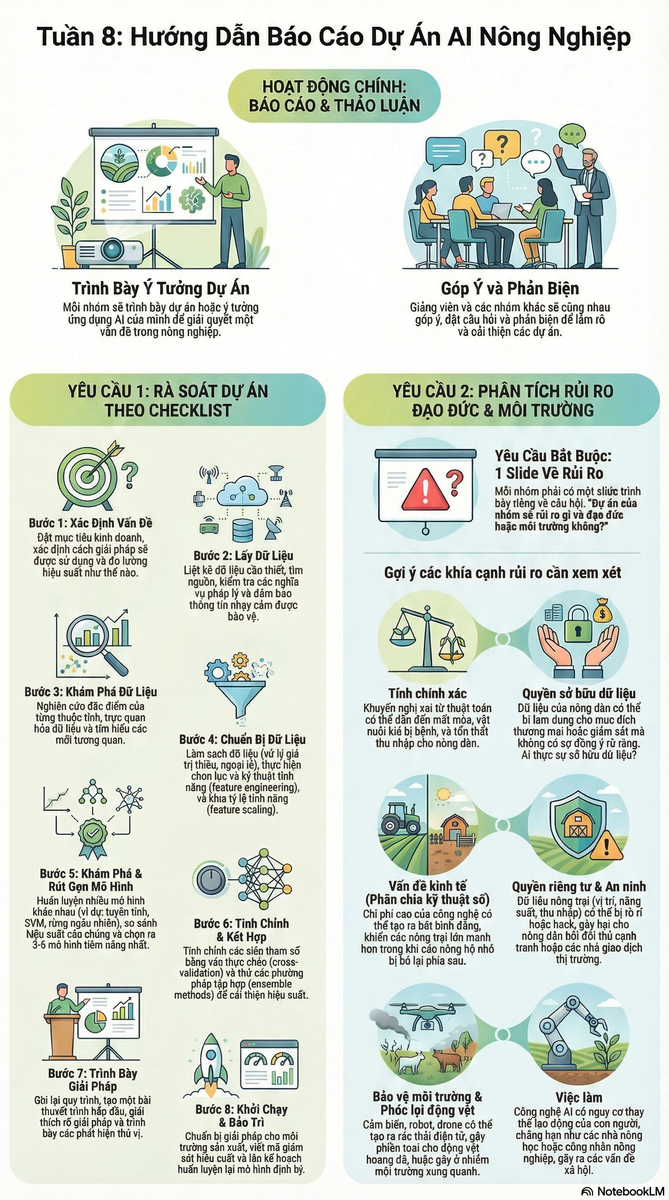
\includegraphics[width=\linewidth,height=0.72\textheight,keepaspectratio]{images_ontap/b8_infographic.png}
        \end{column}
    \end{columns}
\end{frame}

\end{document}
